\documentclass[8pt]{beamer}

%\usetheme{Warsaw}

\usepackage{graphicx}
\usepackage{amsmath}
\usepackage{amsfonts}
\usepackage{amssymb}
\usefonttheme{serif}

\usepackage{mathtext}


\usepackage[T2A]{fontenc}
\usepackage[utf8]{inputenc}
\usepackage[english,ukrainian]{babel} 

\numberwithin{figure}{section}
\numberwithin{equation}{section}
\numberwithin{table}{section}
\setbeamertemplate{caption}[numbered]

\usepackage[justification=centering]{caption}


\title{Амплітудно-частотні характеристики шаруватих пластин і циліндричних оболонок зі складною геометрією напрямної}
\author[Горячко Тарас Всеволодович]{{\large Горячко Тарас Всеволодович}\\[10mm]{\small Науковий керівник: доктор фізико-математичних наук, професор\\ Марчук М.В. }}
\institute{Інститут прикладних проблем механіки і математики ім. Я. С. Підстригача \\ НАН України\\[\medskipamount]
      
\includegraphics[width=0.25\textwidth,height=0.2\textheight]{pic/ilogo.jpg}%
}
\date{}

\begin{document}
\begin{frame}
\titlepage
\end{frame}
\setbeamertemplate{footline}[frame number]

\begin{frame}{Вступ}
\begin{block}{Мета дисертаційної роботи}
Розвиток методу збурень в поєднанні з методом скінченних елементів стосовно задач визначення амплітудно-частотних характеристик шаруватих пластин і циліндричних оболонок з складною геометрією напрямної за лінійних та геометрично  нелінійних коливань.
\end{block}
\begin{block}{Об’єкт дослідження}
Процеси лінійних і геометрично нелінійних коливань шаруватих пластин і циліндричних оболонок зі складною геометрією напрямної.
\end{block}
\begin{block}{Предмет дослідження}
Спектри власних частот та амплітудно-частотні залежності шаруватих пластин і циліндричних оболонок зі складною геометрією напрямної за лінійних та геометрично  нелінійних коливань.
\end{block}
\end{frame}

\begin{frame}{Вступ}

\begin{block}{Публікації та апробації за темою дисертації}
За результатами досліджень опубліковано 17 наукових робіт, із них 5 статей у виданнях з переліку затвердженого ДАК МОН України, 6 статей у збірниках матеріалів наукових конференцій, а також 6 публікацій у збірниках тез наукових конференцій. \\
\textbf{Статті}
\begin{enumerate}
\item Marchuk M., Goriachko T., Pakosh V. Geometrically Nonlinear Free Transversal Vibrations of Thin-Walled Elongated Panels with Arbitrary Generatrix // Vibrations in Physical Systems. – 2014. – Vol. 26. – P. 153–160.
\item Marchuk M., Goriachko T., Pakosh V. Natural Frequencies of Layered Elongated Cylindrical Panels for Geometrically Nonlinear Deformation at Discrete Consideration of Components // Vibrations in Physical Systems. – 2016. – Vol. 27. – P. 255–264.
\end{enumerate}
представлені у провідних світових наукометричних базах, зокрема у Scopus. \linebreak \linebreak
\textbf{Матеріали досліджень доповідались на 12 міжнародних та Всеукраїнських наукових конференціях.}
\end{block}

\end{frame}

\section{Розділ 1}

\begin{frame}{Розділ 1. Основні методи і результати теоретичних досліджень за проблемою визначення  амплітудно-частотних характеристик шаруватих пластин і циліндричних оболонок за лінійного та геометрично нелінійного деформування.}
\textbf{Огляд публікацій за проблемою теоретичного аналізу лінійних і нелінійних коливань оболонок і пластин}\\[3mm]
\indent Дослідження процесів лінійних та нелінійних коливань тонкостінних елементів конструкцій із традиційних матеріалів було започатковано на основі використання класичної теорії, що базується на гіпотезі Кірхгофа-Лява. Фундаментальні результати в цьому напрямку отримані в працях \alert{ В.В. Болотіна, А.С. Вольміра, В.Т. Грінченка, Я.М. Григоренка, В.А. Криська, В.Д. Кубенка, Л.В. Курпи, С.П. Тимошенка та інших учених}. 

\medskip 
Слід відмітити, що такий підхід дозволяє врахувати анізотропію фізико-механічних характеристик лише в тангенціальних напрямках, однак, не дозволяє дослідити вплив на амплітудно частотні характеристики  таких специфічних властивостей нових матеріалів - композитів, як податливість до трансверсальних зсуву та стиснення.

\medskip Суттєві результати у вирішенні цієї проблеми містяться в роботах І. Альтенбаха, С.О. Амбарцумяна, І.М. Векуа, К.З. Галімова, Я.М. Григоренка, О.М. Гузя, В.С. Гудрамовича, Р. Міндліна, П. Нагді, Ю.В. Немировського, Б.Л Пелеха, \alert{І.С. Мухи}, В.Г. Піскунова, Е. Рейснера, М.А. Сухорольського, В.П. Тамужа, С.П. Тимошенка, Л.П. Хорошуна та інших учених.
\end{frame}

\begin{frame}{Розділ 1.}
Дія інтенсивних динамічних (зокрема циклічних) експлуатаційних навантажень спричиняє поперечні переміщення в тонкостінних елементах, котрі співмірні з їхніми товщинами. Це зумовлює геометрично нелінійний характер їх деформованого стану. 
\medskip 

Постановкам задач про лінійній та геометрично нелінійні коливання пластин і оболонок та розробці методів їх розв'язання на основі застосування уточнених теорій присвячені праці О.І. Беспалової, В.В. Болотіна, А.С. Вольміра, В.Т. Грінченка, О.Я. Григоренка, Я.М. Григоренка, В.А. Криська, Л.В. Курпи, М.В. Марчука, Я.Г. Савули, В.І. Сторожева, С.П. Тимошенка, M. Amabili, J Awrejcewicz, I.K. Banerjee, I.C. Chen, Li. A. Dong, C.L. Dym, D.A. Evenren, P.B. Goncalves, E.L. Jansen, L. Librescu, F.M.A. Silva, M. Sundhakar, T. Ueda та інших учених.
\medskip 

Дослідження коливних процесів тонкостінних елементів на основі просторових співвідношень динамічної теорії пружності відображенні \alert{Є. В. Алтухова, Й. І. Воровича, С. Г. Лехницького, Л. С. Плевако, А. К. Приварникова, Р. М. Раппопорт, О. О. Рассказова, В. І. Сторожева, Ю. А. Устінова, В. А. Шалдирвана та ін}.

\medskip 
Розробці та розвиненню методів розв'язування результуючих систем  нелінійних алгебнаїчних рівнянь присвячені роботи \alert{???}


\end{frame}

\section{Розділ 2}

\begin{frame}{Розділ 2. РІВНЯННЯ ДИНАМІЧНО НАПРУЖЕНОГО СТАНУ ЗА ГЕОМЕТРИЧНО НЕЛІНІЙНОГО ДЕФОРМУВАННЯ}

\textbf{2.1. Співвідношення просторової геометрично нелінійної динамічної теорії пружності в криволінійній системі координат.
}

\begin{columns}
	\begin{column}{0.35\linewidth}
		\begin{figure}
			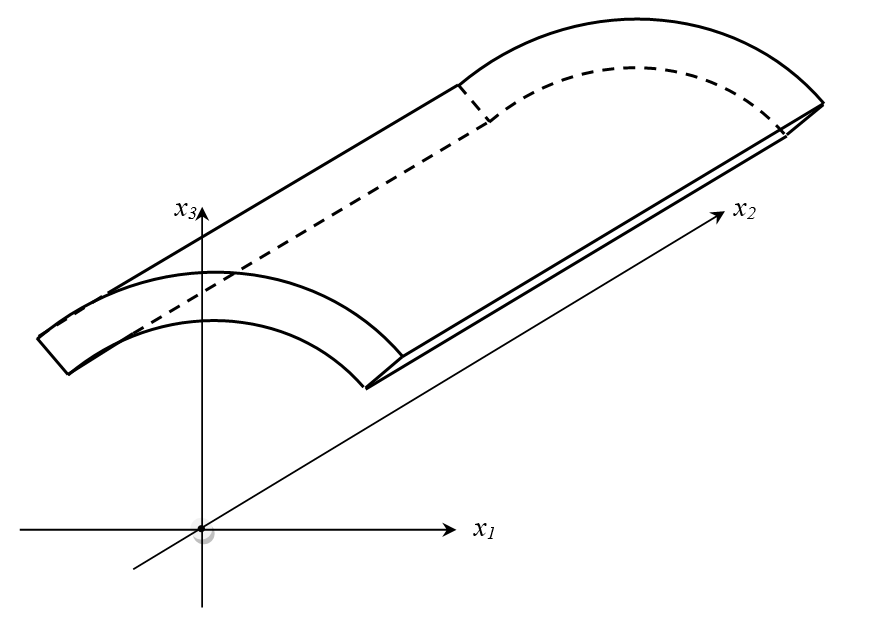
\includegraphics[scale=0.15]{pic/layer.png}
			\caption{Криволінійний пружний шар у декартовій системі координат}
			\label{fig:21}
		\end{figure}
	\end{column}
	\begin{column}{0.65\textwidth}
    	\begin{center}
	    	Напружено-деформований стан описується
    	\end{center}
\begin{align}
\vec{u} &= u^i \vec{R_i}=u_i \vec{R^i},\\
\hat{\varepsilon} &= \varepsilon^{ij} \vec{R_i}\vec{R_j}=\varepsilon_{ij} \vec{R^i}\vec{R^j},\\
\hat{\Sigma} &= \sigma^{ij} \vec{R_i}\vec{R_j}=\sigma_{ij} \vec{R^i}\vec{R^j},\\
\varepsilon_{ij} &= \frac{1}{2} \left( \nabla_i u_j + \nabla_j u_i + \nabla_i u^j \nabla_j u_k \right),\\
\nabla_j u_i &= \frac{ \partial u_i }{ \partial \alpha_j } - u_k G ^k _{ij},\\
G ^k _{ij} &= \frac12 \sum_{m=1}^{3} g^{km} 
\left(
\frac{\partial g_{im}}{\partial \alpha_j} + \frac{\partial g_{jm}}{\partial \alpha_i} - \frac{\partial g_{ij}}{\partial \alpha_m} 
\right), \\
\sigma^{ij} &= C^{ijkm}\varepsilon_{km}.
\end{align}
	\end{column}
\end{columns}


\end{frame}

\begin{frame}{Розділ 2}
\emph{Рівняння руху точок шару}
\begin{equation} \label{eq:P}
div \hat{P} = \rho \frac{\partial^2 \vec{u}}{\partial t^2},
\end{equation}
де $\hat{P}$ --- перший несиметричний тензор Кірхгофа-Піоли, $\rho$ --- скалярне поле, яке визначає густину шару, $t$ --- змінна за часовою координатою.
\linebreak 
\linebreak 
\emph{Граничні умови на лицевих поверхнях}
\begin{equation}
P^{3i}\left( \alpha_1, \alpha_2, \pm \frac{h}{2}, t \right) = X^{\pm}_{3i}\left( \alpha_1, \alpha_2, t \right).
\end{equation}
\linebreak
\emph{Граничні умови на боковій поверхні} $\Omega = \Omega_{\sigma} + \Omega_{u} $
\begin{align}
P^{im}\left( \alpha_1, \alpha_2, \alpha_3, t \right)n_i &= f^{m}\left( \alpha_1, \alpha_2, \alpha_3, t \right), i=1,2,3, m=1,2,3, \left( \alpha_1, \alpha_2,\alpha_3\right)\in\Omega_{\sigma};\\
u^{i}\left( \alpha_1, \alpha_2, \alpha_3, t \right) &=g^{i}\left( \alpha_1, \alpha_2, \alpha_3, t \right), i=1,2,3, \left( \alpha_1, \alpha_2,\alpha_3\right)\in\Omega_{u}.
\end{align}

\emph{Початкові умови}
\begin{equation}
u^{i}\vline _{t=t_0} = u^i_0 \left( \alpha_1, \alpha_2, \alpha_3 \right), \frac{\partial u^{i}}{\partial t}\vline _{t=t_0} =v^i_0 \left( \alpha_1, \alpha_2, \alpha_3 \right), i=1,2,3.
\end{equation}

\end{frame}

\begin{frame}{Розділ 2}
\textbf{2.2. Варіаційна постановка задачі.}
\begin{equation}
\int_{V(t)} \delta\hat{E}:\hat{\tau}\,dV+\int_{V(t)} \rho \delta\vec{u} \frac{\partial^2 \vec{u}}{\partial t ^2}\,dV=\int_{\Omega_\sigma(t)} \delta\vec{u} \vec{f} \,dS ,
\end{equation}

\[
\forall \delta\vec{u} \in D_A 
= \{ 
\vec{u}:\vec{u}\in W_2^{(2)}; 
\vec{u}=\vec{g} \left( \alpha_1, \alpha_2,\alpha_3 \right) \in \Omega_{u}, \forall t \},
\]

\begin{tabbing}
де \= $ W_2^{(2)}$ --- простір Соболєва,\\
\> $\hat{\tau}$ --- тензор напружень Коші,\\
\> $\vec{f}$ --- вектор поверхневих сил,\\
\> $\delta\hat{E}$ --- тензор лінійних деформацій, який відповідає варіації переміщень.
\end{tabbing}
Оскільки $V(t)$ є невідомим, то в початковій (недеформованій) конфігурації
\begin{equation}\label{eq:virtwork_gen}
\int_{V_0} \delta\hat{\varepsilon}:\hat{S}\,dV+\int_{V_0} \rho_0 \delta\vec{u} \frac{\partial^2 \vec{u}}{\partial t ^2}\,dV=\int_{\Omega_{\sigma0}} \delta\vec{u} \vec{f} \,dS,
\end{equation}

\begin{tabbing}
де \= $\hat{S}$ --- другий симетричний тензор напружень Кірхгофа-Піоли, \\для якого справедлива формула $\hat{S} = \hat{P} \left( \hat{F}^{-1} \right)^T $,\\
\> $\hat{P}$ --- тензор з формули \ref{eq:P},\\
\> $\hat{F}=\hat{G} + grad^T \vec{u}$ --- тензор градієнта локального руху,\\
\> $\delta\hat{\varepsilon}$ --- тензор деформацій Гріна, який відповідає варіації переміщень.
\end{tabbing}


\end{frame}

\begin{frame}{Розділ 2}
\textbf{2.3. Компоненти тензора деформацій в довільній системі координат.}
\begin{equation}
\vec{\nabla} \vec{u} =  
B \cdot \tilde{u},
\end{equation}
де \\
\begin{equation}
\vec{\nabla} \vec{u} =  \left(
\nabla_1 u_1  \nabla_2 u_1  \nabla_3 u_1 \nabla_1 u_2  \nabla_2 u_2  \nabla_3 u_2 
\nabla_1 u_3  \nabla_2 u_3  \nabla_3 u_3 
\right)^T,
\end{equation}
\begin{equation}
 \tilde{u} =  \left( u_1 
\frac { \partial u_1 } { \partial \alpha_1} 
\frac { \partial u_1 } { \partial \alpha_2} 
\frac { \partial u_1 } { \partial \alpha_3} 
u_2 
\frac { \partial u_2 } { \partial \alpha_1} 
\frac { \partial u_2 } { \partial \alpha_2} 
\frac { \partial u_2 } { \partial \alpha_3} 
u_3 
\frac { \partial u_3 } { \partial \alpha_1} 
\frac { \partial u_3 } { \partial \alpha_2} 
\frac { \partial u_3 } { \partial \alpha_3} 
\right)^T,
\end{equation}
матриця $B$
\begin{equation}\label{eq:matrixB}
B=
\left[\begin{array}{cccccccccccc}
-G_{11}^1 & 1 & 0 & 0 & -G_{11}^2 & 0 & 0 & 0 & -G_{11}^3 & 0 & 0 & 0\\
-G_{12}^1 & 0 & 1 & 0 & -G_{12}^2 & 0 & 0 & 0 & -G_{12}^3 & 0 & 0 & 0\\
-G_{13}^1 & 0 & 0 & 1 & -G_{13}^2 & 0 & 0 & 0 & -G_{13}^3 & 0 & 0 & 0\\
-G_{21}^1 & 0 & 0 & 0 & -G_{21}^2 & 1 & 0 & 0 & -G_{21}^3 & 0 & 0 & 0\\
-G_{22}^1 & 0 & 0 & 0 & -G_{22}^2 & 0 & 1 & 0 & -G_{22}^3 & 0 & 0 & 0\\
-G_{23}^1 & 0 & 0 & 0 & -G_{23}^2 & 0 & 0 & 1 & -G_{23}^3 & 0 & 0 & 0\\
-G_{31}^1 & 0 & 0 & 0 & -G_{31}^2 & 0 & 0 & 0 & -G_{31}^3 & 1 & 0 & 0\\
-G_{32}^1 & 0 & 0 & 0 & -G_{32}^2 & 0 & 0 & 0 & -G_{32}^3 & 0 & 1 & 0\\
-G_{33}^1 & 0 & 0 & 0 & -G_{33}^2 & 0 & 0 & 0 & -G_{33}^3 & 0 & 0 & 1
\end{array}\right].
\end{equation}

\end{frame}

\begin{frame}{Розділ 2}
Формула для компонент тензора деформацій Гріна
\begin{equation}
\vec{\varepsilon}=\vec{e}+\vec{\eta}=\left(E + E_{NL}^{(1)} \left(\vec {\nabla} \vec{u} \right) \right)\vec {\nabla} \vec{u}=\left(E + E_{NL}^{(2)} \left(\vec {\nabla} \vec{u} \right) \right)\vec {\nabla} \vec{u},
\end{equation}
де 
\begin{align}
\vec{\varepsilon} = \left(
\varepsilon_{11}\,
\varepsilon_{22}\,
\varepsilon_{33}\,
2\varepsilon_{12}\,
2\varepsilon_{13}\,
2\varepsilon_{23}\,
\right)^T,\\
\vec{e} = \left( 
e_{11}\,
e_{22}\,
e_{33}\,
2e_{12}\,
2e_{13}\,
2e_{23}\,
\right)^T,\\
\vec{\eta} = \left( 
\eta_{11}\,
\eta_{22}\,
\eta_{33}\,
2\eta_{12}\,
2\eta_{13}\,
2\eta_{23}\,
\right)^T,
\end{align}
матриця $E$:
\begin{equation}
E=\left[\begin{matrix}1 & 0 & 0 & 0 & 0 & 0 & 0 & 0 & 0\\0 & 0 & 0 & 0 & 1 & 0 & 0 & 0 & 0\\0 & 0 & 0 & 0 & 0 & 0 & 0 & 0 & 1\\0 & 1 & 0 & 1 & 0 & 0 & 0 & 0 & 0\\0 & 0 & 1 & 0 & 0 & 0 & 1 & 0 & 0\\0 & 0 & 0 & 0 & 0 & 1 & 0 & 1 & 0\end{matrix}\right],
\end{equation}


\end{frame}

\begin{frame}{Розділ 2}
матриці $E_{NL}^{(1)}, E_{NL}^{(2)}$:
\begin{equation}
E_{NL}^{(1)}=\left[\begin{matrix}
\frac{\lambda_{11}}{2} & 0 & 0 & \frac{\lambda_{21}}{2} & 0 & 0 & \frac{\lambda_{31}}{2} & 0 & 0\\
0 & \frac{\lambda_{12}}{2} & 0 & 0 & \frac{\lambda_{22}}{2} & 0 & 0 & \frac{\lambda_{32}}{2} & 0\\
0 & 0 & \frac{\lambda_{13}}{2} & 0 & 0 & \frac{\lambda_{23}}{2} & 0 & 0 & \frac{\lambda_{33}}{2}\\
0 & \lambda_{11} & 0 & 0 & \lambda_{21} & 0 & 0 & \lambda_{31} & 0\\
\lambda_{13} & 0 & 0 & \lambda_{23} & 0 & 0 & \lambda_{33} & 0 & 0\\
0 & 0 & \lambda_{12} & 0 & 0 & \lambda_{22} & 0 & 0 & \lambda_{32}
\end{matrix}\right],
\end{equation}
\begin{equation}
E_{NL}^{(2)}=\left[\begin{matrix}
\frac{\lambda_{11}}{2} & 0 & 0 & \frac{\lambda_{21}}{2} & 0 & 0 & \frac{\lambda_{31}}{2} & 0 & 0\\
0 & \frac{\lambda_{12}}{2} & 0 & 0 & \frac{\lambda_{22}}{2} & 0 & 0 & \frac{\lambda_{32}}{2} & 0\\
0 & 0 & \frac{\lambda_{13}}{2} & 0 & 0 & \frac{\lambda_{23}}{2} & 0 & 0 & \frac{\lambda_{33}}{2}\\
\lambda_{12} & 0 & 0 & \lambda_{22} & 0 & 0 & \lambda_{32} & 0 & 0\\
0 & 0 & \lambda_{11} & 0 & 0 & \lambda_{21} & 0 & 0 & \lambda_{31}\\
0 & \lambda_{13} & 0 & 0 & \lambda_{23} & 0 & 0 & \lambda_{33} & 0
\end{matrix}\right],
\end{equation}
де
$ \lambda_{ij}=\sum_k g^{ik}\nabla_j u_k $.

\end{frame}

\begin{frame}{Розділ 2}
\textbf{2.4. Фізичні компоненти переміщень і параметри Ламе.}
\linebreak
\linebreak
Змішана криволінійна ортогональна система координат:
\begin{gather}
g_{11}=H_1^2, g_{22}=H_2^2, g_{33}=1, \\
g_{ij}=0, i,j=1,2,3, i \ne j;
\end{gather}
Довільна циліндрична система координат
\begin{align}
H_1 = H_1 \left( \alpha_1, \alpha_2, \alpha_3 \right) &= A \left( \alpha_1 \right) \left( 1+ \alpha_3 K \left( \alpha_1 \right) \right),  \\
H_2 = H_2 \left( \alpha_1, \alpha_2, \alpha_3 \right) &= 1,
\end{align}

\begin{tabbing}
де \= $  A \left( \alpha_1 \right)$ --- коефіцієнт першої квадратичної форми серединної поверхні оболонки,\\
\> $K \left( \alpha_1 \right)$ --- головна кривина напрямної в напрямку осі $\alpha_1$.
\end{tabbing}
тоді матриця $B$ \eqref{eq:matrixB}
\begin{equation}
B=
\left[\begin{array}{@{}c@{\hspace{-8pt}}c@{\hspace{2pt}}ccc@{\hspace{2pt}}c@{\hspace{2pt}}cc@{\hspace{1pt}}c@{\hspace{-8pt}}c@{\hspace{1pt}}cc}
0 & \frac{1}{A \left(1+ \alpha_{3} K \right)} & 0 & 0 & 0 & 0 & 0 & 0 & \frac{K}{1+ \alpha_{3} K } & 0 & 0 & 0\\0 & 0 & 1 & 0 & 0 & 0 & 0 & 0 & 0 & 0 & 0 & 0\\0 & 0 & 0 & 1 & 0 & 0 & 0 & 0 & 0 & 0 & 0 & 0\\0 & 0 & 0 & 0 & 0 & \frac{1}{A \left(1+ \alpha_{3} K \right)} & 0 & 0 & 0 & 0 & 0 & 0\\0 & 0 & 0 & 0 & 0 & 0 & 1 & 0 & 0 & 0 & 0 & 0\\0 & 0 & 0 & 0 & 0 & 0 & 0 & 1 & 0 & 0 & 0 & 0\\- \frac{K}{1+ \alpha_{3} K } & 0 & 0 & 0 & 0 & 0 & 0 & 0 & 0 & \frac{1}{A \left(1+ \alpha_{3} K \right)} & 0 & 0\\0 & 0 & 0 & 0 & 0 & 0 & 0 & 0 & 0 & 0 & 1 & 0\\0 & 0 & 0 & 0 & 0 & 0 & 0 & 0 & 0 & 0 & 0 & 1\end{array}\right].
\end{equation}

\end{frame}


\begin{frame}{Розділ 2}
\textbf{2.5. Варіаційна постановка задачі відносно переміщень.}
\begin{gather}
\int_{V_0} \delta\hat{\varepsilon}:\hat{S}\,dV=\int_{V_0} \delta\overline{u} ^T B ^T\left( E + E_{NL} \right)^T C \left( E + E_{NL}^{(1)} \right)B \overline{u} \, dV, \\ 
\int_{V_0} \rho_0 \delta\tilde{u} ^T \frac{\partial^2 \tilde{u}}{\partial t ^2}\,dV=\int_{V_0} \rho_0 \delta\overline{u} ^T \tilde{B}^T \tilde{B}\frac{\partial^2 \overline{u}}{\partial t ^2}\,dV.
\end{gather}
Тоді \eqref{eq:virtwork_gen}:
\begin{multline} \label{eq:virtwork_gen_u}
\int_{V_0} \delta\overline{u} ^T B ^T\left( E + E_{NL} \right)^T C \left( E + E_{NL}^{(1)} \right)B \overline{u} \, dV+\\+\int_{V_0} \rho_0 \delta\overline{u} ^T \tilde{B}^T \tilde{B}\frac{\partial^2 \overline{u}}{\partial t ^2}\,dV=F_{out},
\end{multline}
де
\[\tilde{B}=
\left[\begin{array}{cccccccccccc}
1 & 0 & 0 & 0 & 0 & 0 & 0 & 0 & 0 & 0 & 0 & 0\\
0 & 0 & 0 & 0 & 1 & 0 & 0 & 0 & 0 & 0 & 0 & 0\\
0 & 0 & 0 & 0 & 0 & 0 & 0 & 0 & 1 & 0 & 0 & 0
\end{array}\right].
\]


\end{frame}

\begin{frame}{Розділ 2}
\textbf{2.6. Побудова одновимірної моделі на основі двовимірної.}
\linebreak
\linebreak
Апроксимація переміщень $u_1$ та $u_3$, за координатою $\alpha_3$ 
\begin{align}
u_1 \left( \alpha_1, \alpha_3 \right) = u_{10} \left( \alpha_1\right)p_0 \left( \alpha_3\right)+u_{11} \left( \alpha_1\right)p_1 \left( \alpha_3\right)+u_{12} \left( \alpha_1\right)p_2 \left( \alpha_3\right),\\
u_3 \left( \alpha_1, \alpha_3 \right) = u_{30} \left( \alpha_1\right)p_0 \left( \alpha_3\right)+u_{31} \left( \alpha_1\right)p_1 \left( \alpha_3\right)+u_{32} \left( \alpha_1\right)p_2 \left( \alpha_3\right),
\end{align}
де поліноми $p_0$, $p_1$ та $p_2$ мають вигляд
\begin{equation}
p_0 \left( \alpha_3\right) = \frac12-\frac{\alpha_3}{h},
p_1 \left( \alpha_3\right) = \frac12+\frac{\alpha_3}{h},
p_2 \left( \alpha_3\right) = 1-\left(\frac{2\alpha_3}{h}\right)^2,
\end{equation}
$h$ --- товщина шару.
\begin{figure}
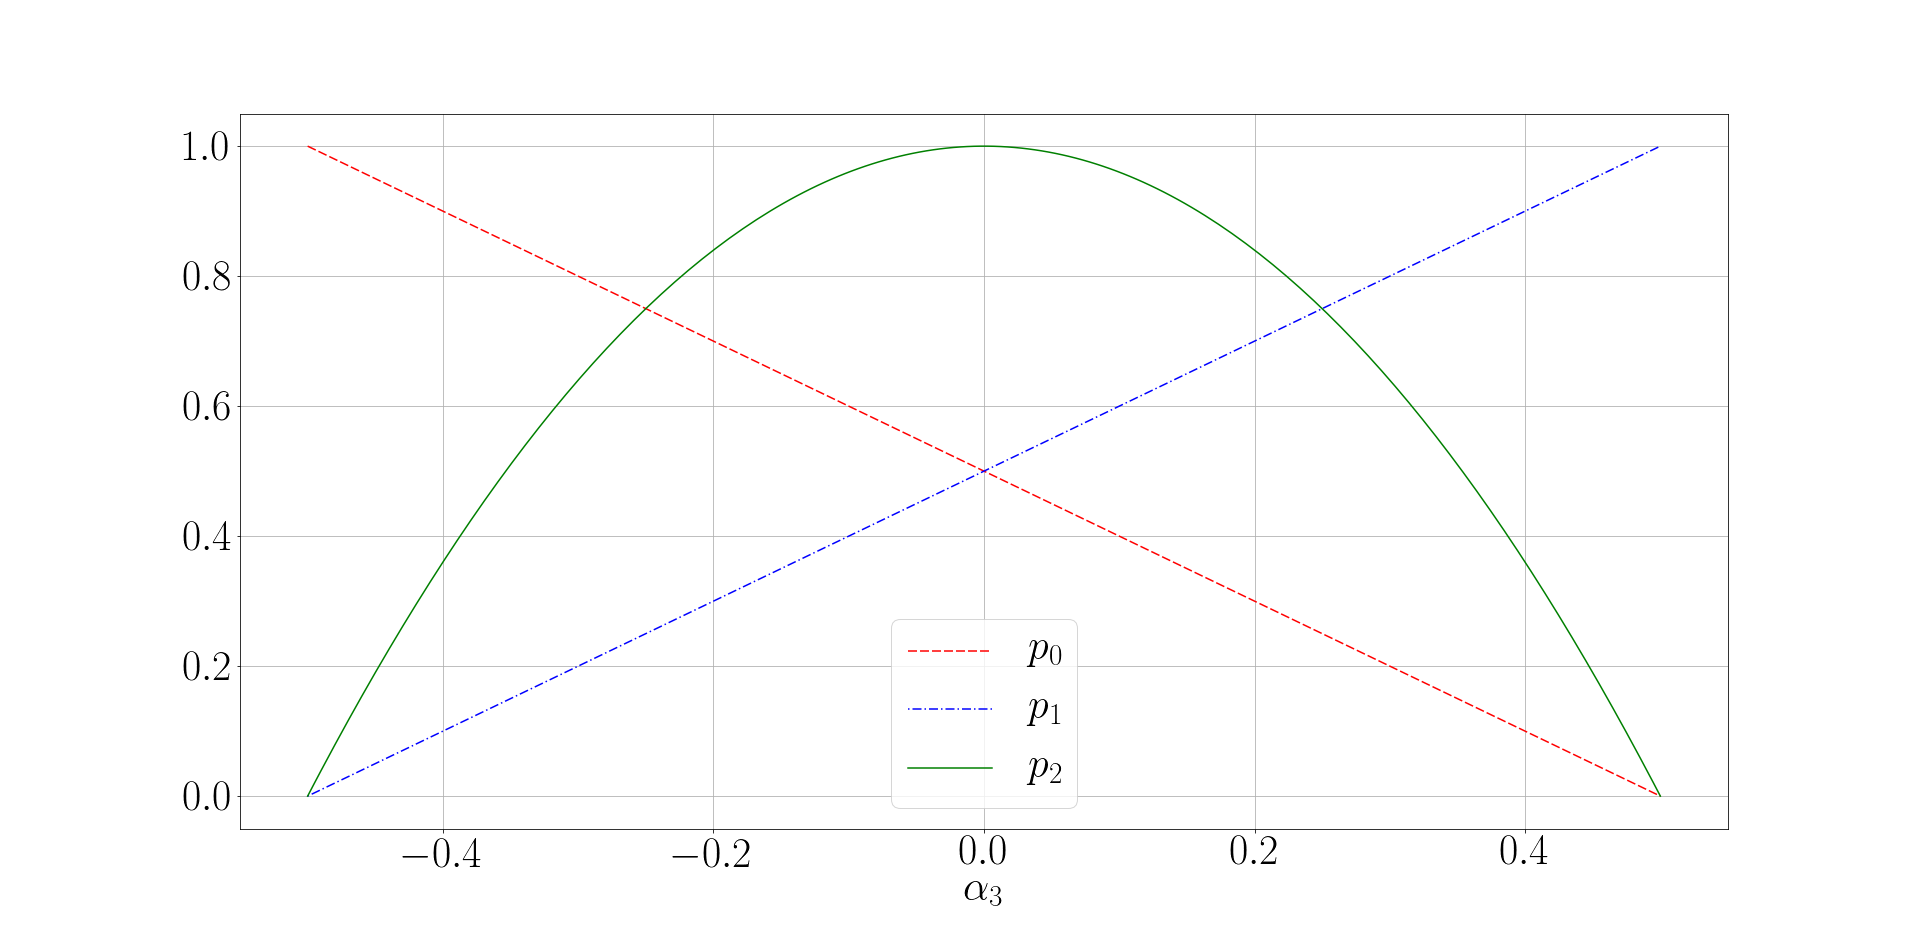
\includegraphics[scale=0.1]{pic/polin.png}
\caption{Графіки поліномів $p_0$, $p_1$ та $p_2$ на проміжку [-0.5;0.5]}
\end{figure}

\end{frame}

\begin{frame}{Розділ 2}
\begin{equation}
\begin{aligned}
&\varepsilon_{ij} \left( \alpha_1, \alpha_3 \right) = \frac{\varepsilon_{ij0} \left( \alpha_1\right)p_0 \left( \alpha_3\right)+\varepsilon_{ij1} \left( \alpha_1\right)p_1 \left( \alpha_3\right)+\varepsilon_{ij2} \left( \alpha_1\right)p_2 \left( \alpha_3\right)}{1+\alpha_3 K},\\
&\varepsilon_{ijk} = e_{ijk}\left( \alpha_1\right)+\eta_{ijk}\left( \alpha_1\right), \quad i,j=1,3, k=0,1,2,
\end{aligned}
\end{equation}

\begin{tabbing}
де \= $e_{ijk}\left( \alpha_1\right)$ --- лінійна складова,\\
\> $\eta_{ijk}\left( \alpha_1\right)$ --- нелінійна складова.
\end{tabbing}



\end{frame}

\begin{frame}{Розділ 2}
\begin{equation}\label{eq:sqt_strain_l}
\begin{aligned}
&e_{11k}\left(\alpha_1\right)=\frac{1}{A\left(\alpha_1\right)}\frac{du_{1k}}{d\alpha_1}+u_{3k}K\left(\alpha_1\right), k=0,1,2,
\\
&\begin{split}
e_{130}\left(\alpha_1\right)=u_{10}\left( -\frac{1}{h}-\frac{K\left( \alpha_1 \right)}{2} \right)+u_{11}\left( \frac{1}{h}-\frac{K\left( \alpha_1 \right)}{2} \right)+ \\ +u_{12}\left( \frac{4}{h}-2K\left( \alpha_1 \right) \right) + \frac{1}{A\left(\alpha_1\right)}\frac{du_{30}}{d\alpha_1},
\end{split}\\
&\begin{split}
e_{131}\left(\alpha_1\right)=u_{10}\left( -\frac{1}{h}-\frac{K\left( \alpha_1 \right)}{2} \right)+u_{11}\left( \frac{1}{h}-\frac{K\left( \alpha_1 \right)}{2} \right)+\\+u_{12}\left( - \frac{4}{h}-2K\left( \alpha_1 \right) \right) + \frac{1}{A\left(\alpha_1\right)}\frac{du_{31}}{d\alpha_1},
\end{split}\\
&e_{132}\left(\alpha_1\right)=\frac{1}{A\left(\alpha_1\right)}\frac{du_{32}}{d\alpha_1}+u_{12}K\left(\alpha_1\right),\\
&\begin{split}
e_{330}\left(\alpha_1\right)=u_{30}\left( -\frac{1}{h}+\frac{K\left( \alpha_1 \right)}{2} \right)+u_{31}\left( \frac{1}{h}-\frac{K\left( \alpha_1 \right)}{2} \right)+\\+u_{32}\left( \frac{4}{h}-2K\left( \alpha_1 \right) \right),
\end{split}\\
&\begin{split}
e_{331}\left(\alpha_1\right)=u_{30}\left( -\frac{1}{h}-\frac{K\left( \alpha_1 \right)}{2} \right)+u_{31}\left( \frac{1}{h}+\frac{K\left( \alpha_1 \right)}{2} \right)+\\+u_{32}\left( -\frac{4}{h}-2K\left( \alpha_1 \right) \right),
\end{split}\\
&e_{332}\left(\alpha_1\right)=2K\left( \alpha_1 \right)u_{32}.
\end{aligned}
\end{equation}
\end{frame}

\begin{frame}{Розділ 2}
\begin{equation}
\begin{aligned}
&\eta_{iik}\left(\alpha_1\right)=\left[\begin{array}{ccc}
\omega_{20} & \omega_{21} & \omega_{22}
\end{array} \right] \Theta_k\left(\alpha_1\right) \left[\begin{array}{ccc}
\omega_{20} & \omega_{21} & \omega_{22}
\end{array} \right]^T,\\
&\eta_{13k}\left(\alpha_1\right)=0, \quad k=0,1,2, i=1,3,
\end{aligned}
\end{equation}
де
\begin{equation}\label{eq:sqt_strain_nl}
\begin{aligned}
\Theta_0\left(\alpha_1\right)=\frac{1}{32}
\left[
\begin{array}{ccc}
16+6Kh+K^2h^2 & 4Kh+2K^2h^2 & 16+16Kh+4K^2h^2 \\ 
4Kh+2K^2h^2 & -2Kh+K^2h^2 & -16Kh+4K^2h^2 \\ 
16+16Kh+4K^2h^2 & -16Kh+4K^2h^2 & -16+8Kh+4K^2h^2
\end{array}
\right],\\
\Theta_1\left(\alpha_1\right)=\frac{1}{32}
\left[
\begin{array}{ccc}
2Kh+K^2h^2 & -4Kh+2K^2h^2 & -16+4K^2h^2 \\ 
-4Kh+2K^2h^2 & 16-6Kh+K^2h^2 & 16-16Kh+4K^2h^2 \\ 
-16+4K^2h^2  & 16-16Kh+4K^2h^2 & -16-8Kh+4K^2h^2
\end{array}
\right],\\
\Theta_2\left(\alpha_1\right)=\frac{1}{32}
\left[
\begin{array}{ccc}
-4-4Kh-K^2h^2 & 8-2K^2h^2 & 16-8Kh-K^2h^2 \\ 
8-2K^2h^2 & -4+4Kh-K^2h^2 & 16+8Kh-4K^2h^2 \\ 
16+16Kh+4K^2h^2 & 16+8Kh-4K^2h^2 & 32-4K^2h^2
\end{array}
\right],\\
\end{aligned}
\end{equation}

\end{frame}

\begin{frame}{Розділ 2}
\begin{equation}\label{eq:sqt_strain_ang}
\begin{aligned}
\omega_{20}\left(\alpha_1\right)=\frac12 
\left[
u_{10}
\left( -\frac{1}{h}+\frac{3K\left( \alpha_1 \right)}{2} \right)
+u_{11}\left( \frac{1}{h}-\frac{K\left( \alpha_1 \right)}{2} \right)+\right.\\
\left.
+u_{12}\left( \frac{4}{h}-2K\left( \alpha_1 \right) \right)
 - \frac{1}{A\left(\alpha_1\right)}\frac{du_{30}}{d\alpha_1}
\right],\\
\omega_{21}\left(\alpha_1\right)=\frac12 
\left[
-u_{10}
\left( \frac{1}{h}+\frac{K\left( \alpha_1 \right)}{2} \right)
+u_{11}\left( \frac{1}{h}+\frac{3K\left( \alpha_1 \right)}{2} \right)-\right.\\
\left.
-u_{12}\left( \frac{4}{h}+2K\left( \alpha_1 \right) \right)
 - \frac{1}{A\left(\alpha_1\right)}\frac{du_{31}}{d\alpha_1}
\right],\\
\omega_{22}\left(\alpha_1\right)=\frac12 
\left[3K\left( \alpha_1 \right)u_{12}
 - \frac{1}{A\left(\alpha_1\right)}\frac{du_{30}}{d\alpha_1}
\right].
\end{aligned}
\end{equation}

\end{frame}

\begin{frame}{Розділ 2}
Тоді \eqref{eq:virtwork_gen}:
\begin{multline}
\int_0^L \delta\overline{u}'^T \left( E' + E_{NL}' \right)^T C' \left( E' + E_{NL}'^{(1)} \right)\overline{u}' A\left(\alpha_1\right)\, d\alpha_1+\\+\int_0^L \rho_0 \delta\overline{u}'^T B'\frac{\partial^2 \overline{u}'}{\partial t^2} A\left(\alpha_1\right)\, d\alpha_1=F_{out}.
\end{multline}
де
\[
\overline{u}' = \left( u_{10}
\frac { du_{10}} { d \alpha_1}
u_{11} 
\frac { du_{11}} { d \alpha_1}
u_{12}
\frac { du_{12}} { d \alpha_1} 
u_{30}
\frac { du_{30}} { d \alpha_1}
u_{31} 
\frac { du_{31}} { d \alpha_1}
u_{32}
\frac { du_{32}} { d \alpha_1} 
\right)^T,
\]


\[
C'=\left[
\begin{array}{ccc}
C'_{11} & C'_{13} & 0 \\ 
C'_{13} & C'_{33} & 0 \\ 
0 & 0 & C'_{55}
\end{array} 
\right], \quad 
C'_{ij}=hC_{ij}\left[
\begin{array}{ccc}
1/3 & 1/6 & 1/3 \\ 
1/6 & 1/3 & 1/3 \\ 
1/3 & 1/3 & 8/15
\end{array} 
\right], i,j=1,3,5,
\]

\[
B'=\left[
\begin{array}{cc}
B'_0 & 0 \\ 
0 & B'_0
\end{array} 
\right], \quad 
B'_0=h\left[
\begin{array}{cccccc}
1/3 & 0 & 1/6 & 0 & 1/3 & 0 \\ 
0 & 0 & 0 & 0 & 0 & 0 \\ 
1/6 & 0 & 1/3 & 0 & 1/3 & 0 \\ 
0 & 0 & 0 & 0 & 0 & 0 \\ 
1/3 & 0 & 1/3 & 0 & 8/15 & 0\\
0 & 0 & 0 & 0 & 0 & 0 
\end{array} 
\right],
\]

матриці $E'$, $E_{NL}'$ та $E_{NL}'^{(1)}$ побудовані з \eqref{eq:sqt_strain_l}, \eqref{eq:sqt_strain_nl} та \eqref{eq:sqt_strain_ang}.

\end{frame}
\begin{frame}{Розділ 2}
\textbf{Висновки до розділу 2}\\
\vspace{1em}
\begin{itemize}
\item У розділі розглянута загальна диференціальна постановка задачі про динамічний напружено-деформований стан ортотропного криволінійного шару за геометрично нелінійного деформування.
\item На цій основі зроблено постановку еквівалентної варіаційної задачі в компонентах апроксимацій переміщень.
\item Проаналізовано та досліджено структуру побудованого функціоналу.
\item Отримані основні співвідношення вказаного методу з врахуванням особливості побудованого фунціоналу.
\item Шляхом апроксимації компонент вектора переміщень за нормальною до серединної поверхні шару координатою по запропонованим співвідношенням отримано одновимірну варіаційну задачу. 
\end{itemize}

\end{frame}

\section{Розділ 3}
\begin{frame}{Розділ 3. УЗАГАЛЬНЕНИЙ МЕТОД ЗБУРЕНЬ У ЗАДАЧАХ ПРО КОЛИВАННЯ}
\textbf{3.1. Скінченно-елементні апроксимації для двовимірних моделей коливань товстостінних і тонкостінних оболонок і пластин.}
\\
\vspace{1em}
\begin{equation}
V=\bigcup\limits_{e=1}^{NM} V^{(e)}.
\end{equation}
Тоді \eqref{eq:virtwork_gen_u}
\begin{equation}
\sum_{e=1}^{NM}\int_{V^{(e)}}  \left[ \delta\overline{u} ^T B ^T\left( E + E_{NL} \right)^T C \left( E + E_{NL}^{(1)} \right)B \overline{u} + \rho_0 \delta\overline{u} ^T \tilde{B}^T \tilde{B}\frac{\partial^2 \overline{u}}{\partial t ^2} \right] \,dV=0.
\end{equation}
Апроксимації переміщень на скінченному елементі $V^{(e)}$
\begin{equation}
\begin{aligned}
\varphi_0&=\frac{1}{4}\left(1-\xi\right)\left(1+\eta\right) & \varphi_1 &=\frac{1}{4}\left(1+\xi\right)\left(1+\eta\right)\\
\varphi_2&=\frac{1}{4}\left(1+\xi\right)\left(1-\eta\right) & \varphi_3 &=\frac{1}{4}\left(1-\xi\right)\left(1-\eta\right)
\end{aligned}
\end{equation}
де $\xi \in [-1;1], \eta \in [-1;1]$.

\end{frame}

\begin{frame}{Розділ 3}
\begin{equation}
K_L\overline{U}+\left( K_{NL}^{(1)}\left( \overline{U}\right)+K_{NL}^{(2)}\left( \overline{U},\overline{U}\right) \right)\overline{U}+M\ddot{\overline{U}}=0,
\end{equation}
де 
\begin{gather}
M=\sum_{e=1}^{NM}
\left[ \int\limits_{-1}^{1} \int\limits_{-1}^{1} \rho_0 {H^{(e)}}^T \tilde{B}^T \tilde{B} H^{(e)} J^{(e)} \, d\xi \, d\eta \right],\\
K_L=\sum_{e=1}^{NM}
\left[ \int\limits_{-1}^{1} \int\limits_{-1}^{1} {H^{(e)}}^T B^T E^T C E B H^{(e)} J^{(e)} \, d\xi \, d\eta \right],\\
K_{NL}^{(1)}=\sum_{e=1}^{NM}
\left[ 
\begin{aligned}
\int\limits_{-1}^{1} \int\limits_{-1}^{1} {H^{(e)}}^T B^T E_{NL}\left( \overline{U}\right)^T C E B H^{(e)} J^{(e)} \, d\xi \, d\eta + \\ 
+ \int\limits_{-1}^{1} \int\limits_{-1}^{1} {H^{(e)}}^T B^T E^T C E_{NL}^{(1)}\left( \overline{U}\right) B H^{(e)} J^{(e)} \, d\xi \, d\eta 
\end{aligned} 
\right],\\
K_{NL}^{(2)}=\sum_{e=1}^{NM}
\left[ 
\int\limits_{-1}^{1} \int\limits_{-1}^{1} {H^{(e)}}^T B^T E_{NL}\left( \overline{U}\right)^T C E_{NL}^{(1)}\left( \overline{U}\right) B H^{(e)} J^{(e)} \, d\xi \, d\eta 
\right].
\end{gather}

\end{frame}

\begin{frame}{Розділ 3}
\textbf{3.3. Метод скінченних елементів стосовно одновимірної моделі.}
\\
\vspace{1em}
\begin{equation}
V=\bigcup\limits_{e=1}^{N} V^{(e)}.
\end{equation}
Апроксимації переміщень на одновимірному скінченному елементі $V^{(e)} = [\alpha_{1s};\alpha_{1e}]$
\begin{equation}
\begin{aligned}
\varphi_0&=\frac{1}{2}\left(1-\xi\right) & \varphi_1 &=\frac{1}{2}\left(1+\xi\right)
\end{aligned}
\end{equation}
де $\xi \in [-1;1]$.
\end{frame}

\begin{frame}{Розділ 3}
\begin{equation}
K'_L\overline{U}'+\left( K_{NL}'^{(1)}\left( \overline{U}'\right)+K_{NL}'^{(2)}\left( \overline{U}',\overline{U}'\right) \right)\overline{U}'+M'\ddot{\overline{U}}'=0,
\end{equation}
де 
\begin{gather}
M'=\sum_{e=1}^{N}
\left[ \int\limits_{-1}^{1} \rho_0 {H'^{(e)}}^T B' H'^{(e)} J'^{(e)} A\left(\xi\right) \, d\xi \right],\\
K'_L=\sum_{e=1}^{N}
\left[ \int\limits_{-1}^{1}{H'^{(e)}}^T E'^T C' E' H'^{(e)} J'^{(e)} A\left(\xi\right) \, d\xi \right],\\
K_{NL}'^{(1)}=\sum_{e=1}^{N}
\left[ 
\begin{aligned}
\int\limits_{-1}^{1} {H'^{(e)}}^T E'_{NL}\left( \overline{U}'\right)^T C' E' H'^{(e)} J'^{(e)} A\left(\xi\right) \, d\xi  + \\ 
+ \int\limits_{-1}^{1} {H'^{(e)}}^T E'^T C' E_{NL}'^{(1)}\left( \overline{U}'\right) H'^{(e)} J'^{(e)} A\left(\xi\right) \, d\xi 
\end{aligned} 
\right],\\
K_{NL}^{(2)}=\sum_{e=1}^{NM}
\left[ 
\int\limits_{-1}^{1} \int\limits_{-1}^{1} {H^{(e)}}^T B^T E_{NL}\left( \overline{U}\right)^T C E_{NL}^{(1)}\left( \overline{U}\right) B H^{(e)} J^{(e)} \, d\xi \, d\eta 
\right].
\end{gather}

\end{frame}

\begin{frame}{Розділ 3}
\textbf{3.4. Узагальнення методу збурень до розв’язання результуючої системи нелінійних алгебраїчних рівнянь.}
\begin{equation}\label{eq:nonlineq}
K_L\overline{U}+\mu \left( K_{NL}^{(1)}\left( \overline{U}\right)+K_{NL}^{(2)}\left( \overline{U},\overline{U}\right) \right)\overline{U}+M\ddot{\overline{U}}=0,
\end{equation}
де $\mu \in [0;1]$ --- параметр збурення.
\begin{equation}
\overline{U}\left(t\right) =\overline{U}_0\left(t\right) + \mu \overline{U}_1\left(t\right) + O\left( \mu^2\right).
\end{equation}
Секулярний член
\begin{equation}
\overline{U}_S\left(t\right) =\begingroup\color{red}t\endgroup \sin \omega t.
\end{equation}
Узагальнення методу збурень
\begin{equation}
K_L = K - \mu K_{L1} + O\left( \mu^2\right).
\end{equation}
Початкові умови
\begin{align}
\overline{U}\vline _{t=t_0}=\overline{A}\approx A\overline{\phi},\qquad \dot{\overline{U}}\vline _{t=t_0}=\overline{0}.
\end{align}
де $\overline{\phi}$ --- власний вектор лінійної задачі, для якого
\begin{equation}\label{eq:lin_prop}
\begin{aligned}
\overline{\phi}^T K_L \overline{\phi} &= \omega_L^2 , \\
\overline{\phi}^T M \overline{\phi} &= 1 .
\end{aligned}
\end{equation}
\end{frame}

\begin{frame}{Розділ 3}
\begin{gather}
\label{eq:firstU0}
K\overline{U}_0+M\ddot{\overline{U}}_0=0,\\
\label{eq:firstU1}
K\overline{U}_1+M\ddot{\overline{U}}_1=K_{L1}\overline{U}_0-K_{NL}^{(1)}\left( \overline{U}_0 \right) \overline{U}_0-K_{NL}^{(2)}\left( \overline{U}_0,\overline{U}_0\right)\overline{U}_0.
\end{gather}
Розв'язок \eqref{eq:firstU0}
\begin{equation}
\overline{U}_0=A\overline{\phi}\cos\omega t.
\end{equation}
Тоді з \eqref{eq:lin_prop}
\begin{equation}
\omega^2=\overline{\phi}^T K \overline{\phi}.
\end{equation}

Використавши
\begin{equation}
\cos^2 \omega t = \frac12 + \frac12 \cos 2 \omega t , \quad
\cos^3 \omega t = \frac34 \cos \omega t + \frac14 \cos 3 \omega t,
\end{equation}
і представивши
\begin{equation}
K_{L1} = \frac34 K_{NL}^{(2)}\left( A\overline{\phi},A\overline{\phi} \right),
\end{equation}
Рівняння \eqref{eq:firstU1}:
\begin{multline}\label{eq:secondU1}
K\overline{U}_1+M\ddot{\overline{U}}_1=-\frac12 K_{NL}^{(1)}\left( A\overline{\phi} \right) A\overline{\phi} -\frac12 K_{NL}^{(1)}\left( A\overline{\phi} \right) A\overline{\phi} \cos 2\omega t -\\ - \frac14 K_{NL}^{(2)}\left( A\overline{\phi},A\overline{\phi}\right)A\overline{\phi} \cos 3\omega t.
\end{multline}

\end{frame}


\begin{frame}{Розділ 3}
Розв'язки \eqref{eq:secondU1}:
\begin{align}
\overline{U}_1^{(1)}&=x_1\overline{\phi},\\
\overline{U}_1^{(2)}&=x_2\overline{\phi}\cos 2\omega t,\\
\overline{U}_1^{(3)}&=x_3\overline{\phi}\cos 3\omega t,
\end{align}
де
\begin{align}
x_1&=-\frac{1}{2\omega ^2}\overline{\phi}^T K_{NL}^{(1)}\left( A\overline{\phi} \right) A\overline{\phi},\\
x_2&=\frac{1}{6\omega ^2}\overline{\phi}^T K_{NL}^{(1)}\left( A\overline{\phi} \right) A\overline{\phi},\\
x_3&=\frac{1}{32\omega ^2}\overline{\phi}^T K_{NL}^{(2)}\left( A\overline{\phi},A\overline{\phi} \right) A\overline{\phi},
\end{align}
Загальний розв'язок \eqref{eq:nonlineq}:
\begin{equation}
\overline{U}\left(t\right)=\left[\left(A-x_1-x_2-x_3\right)\cos \omega t + x_1+x_2\cos 2 \omega t+x_3\cos 3 \omega t\right]\overline{\phi}.
\end{equation}
\end{frame}

\begin{frame}{Розділ 3}
Алгоритм відшукання розв'язку:
\begin{enumerate}
	\item Розв’язання лінійної задачі:
	$K_L\overline{\phi}+\omega_L^2 M \overline{\phi}=0$.
 
	\item Апроксимація початкової умови $\overline{A}\approx A\overline{\phi}$: 
	$\displaystyle A=\min_{C \in R} ||\overline{A}-C\overline{\phi}||$.
	\item Обчислення матриці:
	$K = K_L + \frac34 K_{NL}^{(2)}\left( A\overline{\phi},A\overline{\phi} \right) $.
	\item Знаходження власної частоти $\omega$ геометрично нелінійних коливань:
	\[\omega^2=\overline{\phi}^T K \overline{\phi}.\]
	\item Визначення амплітуд:
 \begin{align*}
x_1&=-\frac{1}{2\omega ^2}\overline{\phi}^T K_{NL}^{(1)}\left( A\overline{\phi} \right) A\overline{\phi},\\
x_2&=\frac{1}{6\omega ^2}\overline{\phi}^T K_{NL}^{(1)}\left( A\overline{\phi} \right) A\overline{\phi},\\
x_3&=\frac{1}{32\omega ^2}\overline{\phi}^T K_{NL}^{(2)}\left( A\overline{\phi},A\overline{\phi} \right) A\overline{\phi}.
\end{align*}
	\item Наближений розв'язок:
	\[
	\overline{U}\left(t\right)=\left[\left(A-x_1-x_2-x_3\right)\cos \omega t + x_1+x_2\cos 2 \omega t+x_3\cos 3 \omega t\right]\overline{\phi}.
	\]
\end{enumerate}
\end{frame}

\begin{frame}{Розділ 3}
\textbf{3.6. Висновки до розділу 3}
\\
\vspace{1em}
\begin{itemize}
\item На основі застосування двовимірної схеми МСЕ отримано у матричному вигляді системи нелінійних алгебраїчних рівнянь відносно векторів вузлових переміщень, через які визначаються амплітудно-частотні характеристики криволінійного пружного шару.
\item Аналогічним чином застосовано МСЕ до одновимірної варіаційної задачі та отримано однотипну систему нелінійних алгебраїчних рівнянь.
\item Виведені аналітичні формули для коефіцієнтів лінійних і нелінійних матриць жорсткості та мас, які дозволяють проводити їх швидке обчислення.
\item Для розв'язання отриманих систем узагальнено метод збурень.
\item На цій основі розроблено алгоритм знаходження скінченної кількості перших форм і значень власних частот. 
\end{itemize}

\end{frame}

\section{Розділ 4}
\begin{frame}{Розділ 4. ВІЛЬНІ КОЛИВАННЯ ПЛАСТИН СМУГ ТА ВИДОВЖЕНИХ ЦИЛІНДРИЧНИХ ПАНЕЛЕЙ}
\textbf{4.1. Пластина-смуга}
\begin{equation}
A\left( \alpha_1 \right)=1, \quad K\left( \alpha_1 \right)=0.
\end{equation}
\textbf{\textit{4.1.1 Одношарова пластина-смуга}}
\vspace{1em}

Геометричні та механічні  параметри

\begin{gather*}
l=1\text{м}, h=0.1\text{м},\\
E_1=E, v_{13}=v_{31}=0.3, G_{13}=G;
\end{gather*}

\begin{figure}
	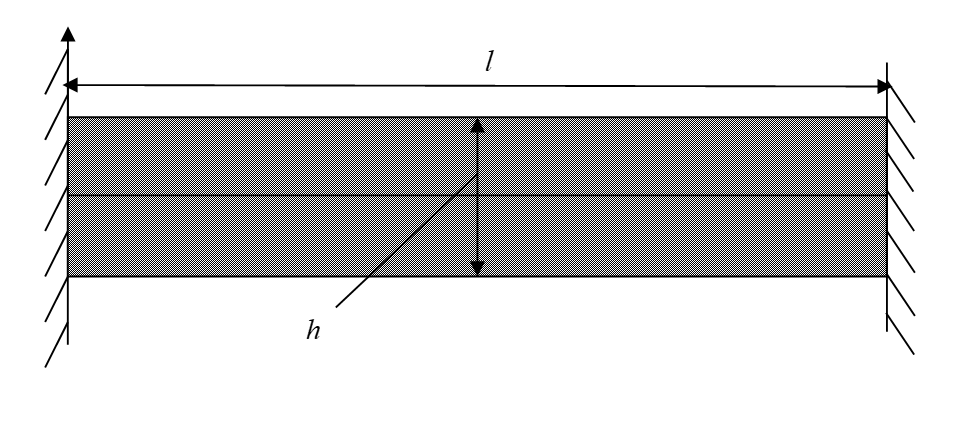
\includegraphics[scale=0.3]{pic/plate.png}
		\caption{Пластина-смуга з защемленими краями}
		\label{fig:plate}
\end{figure}



\end{frame}

\begin{frame}{Розділ 4}

\textbf{\textit{4.1.1.1 Лінійні коливання}}

\begin{figure}
	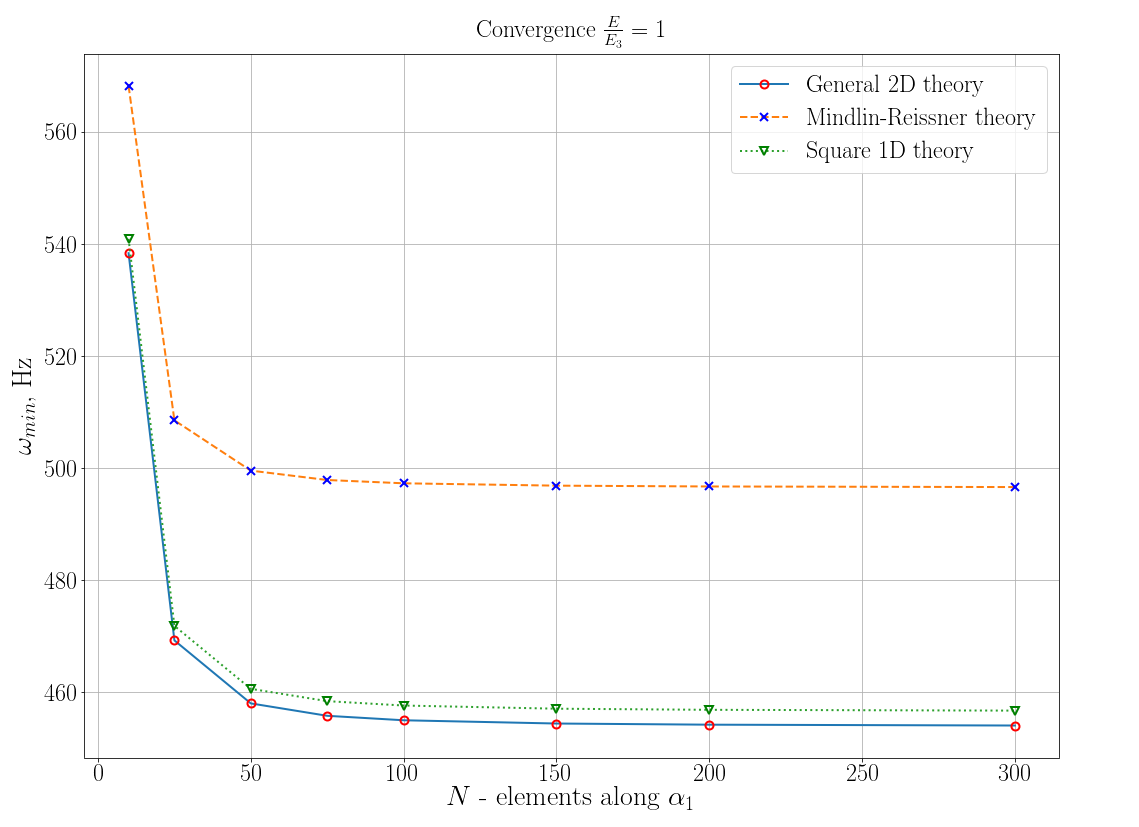
\includegraphics[scale=0.23]{pic/conv_all.png}
		\caption{Збіжність значення мінімальної частоти при збільшенні кількості скінченних елементів вздовж осі $\alpha_3$ з врахуванням стиснення $\frac{E_1}{E_3}\rightarrow1$}
		\label{fig:EE31}
\end{figure}

\end{frame}

\begin{frame}{Розділ 4}
\begin{figure}
	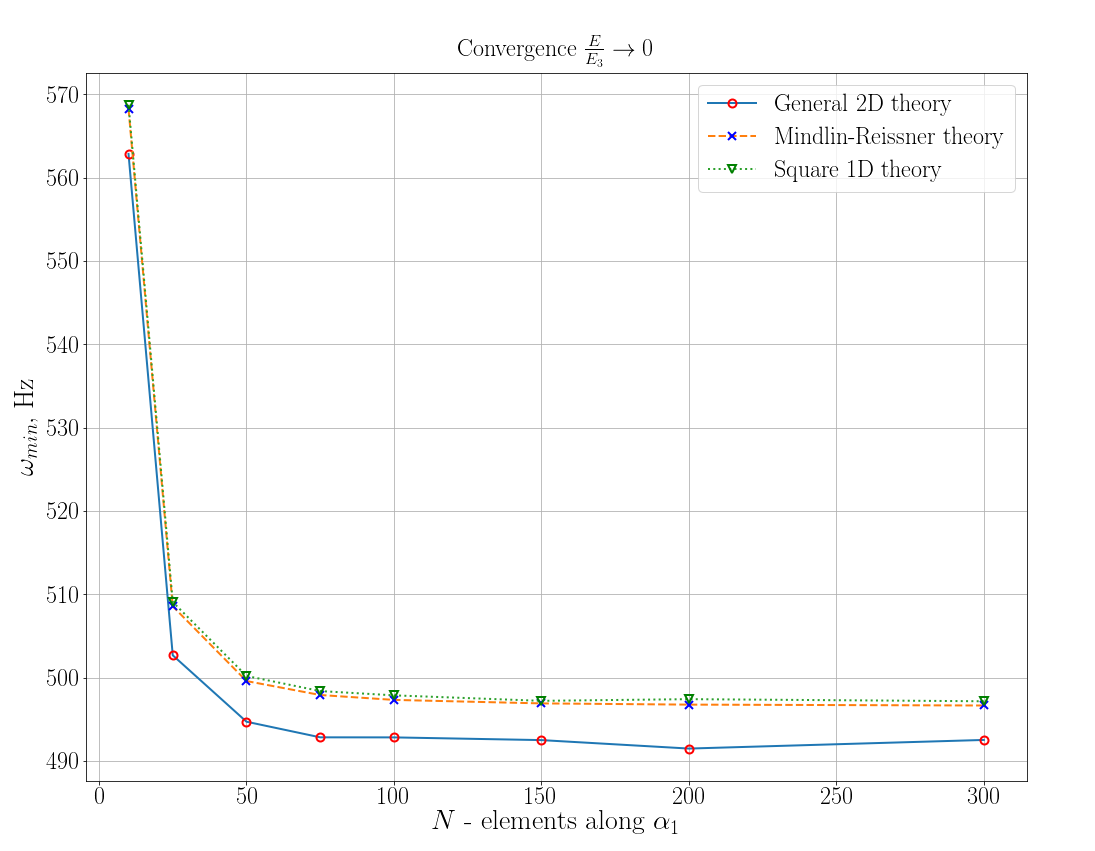
\includegraphics[scale=0.23]{pic/conv_all_e3.png}
		\caption{Збіжність значення мінімальної частоти при збільшенні кількості скінченних елементів вздовж осі $\alpha_3$ без врахування стиснення $\frac{E_1}{E_3}\rightarrow0$}
		\label{fig:EE30}
\end{figure}

\end{frame}

\begin{frame}{Розділ 4}
\begin{figure}
	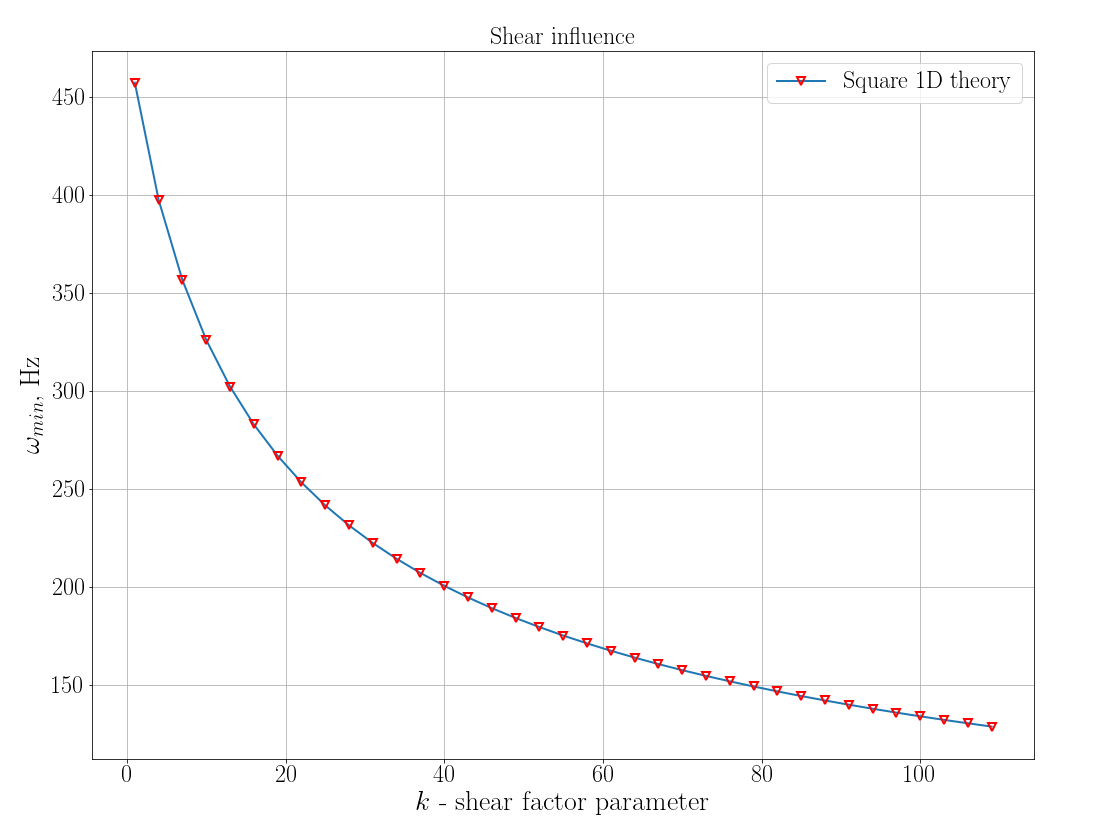
\includegraphics[scale=0.23]{pic/shear_inf.png}
		\caption{Вплив значення модуля трансверсального зсуву на власну мінімальну частоту $G_{13}=\frac{G}{k}$}
		\label{fig:shear}
\end{figure}

\end{frame}

\begin{frame}{Розділ 4}

\textbf{\textit{4.1.1.2 Геометрично нелінійні коливання}}
\begin{figure}
	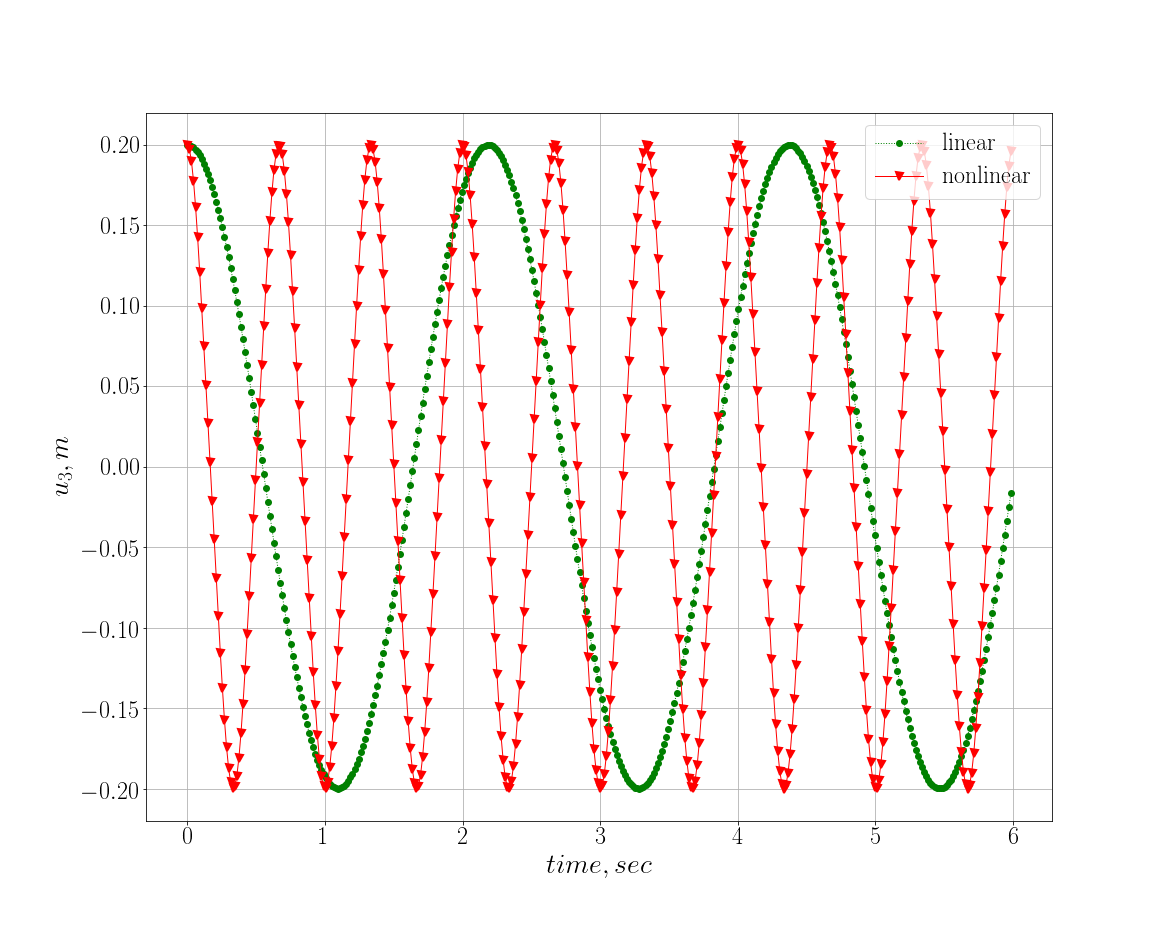
\includegraphics[scale=0.2]{pic/lin_nonlin_time_w2h.png}
		\caption{Лінійні ($\bullet $) і нелінійні ($ \triangledown $) вільні коливання точки панелі з координатами $(\frac{l}{2};0)$ при $w_{max}=2h$.}
		\label{fig:nonlin_time}
\end{figure}

\end{frame}

\begin{frame}{Розділ 4}
Співвідношення для визначення власної частоти геометрично нелінійних вільних коливань
\begin{equation}
\omega^2=\overline{\phi}^T K \overline{\phi}, \quad K = K_L + \frac34 K_{NL}^{(2)}\left( A\overline{\phi},A\overline{\phi} \right).
\end{equation}

Тоді
\begin{equation}
\omega^2=\omega_0^2\left(1+\frac{3}{4}R\left(\frac{w_{max}}{h}\right)^2\right)
\end{equation}

\begin{tabbing}
де \= $\omega_0^2$ --- лінійна власна частота,\\
\> $\omega^2$ --- нелінійна власна частота.
\end{tabbing}

\begin{equation}
R=\frac{\overline{\phi}^T K_{NL}^{(2)}\left( h\overline{\phi}',h\overline{\phi}' \right) \overline{\phi}}{\omega_0^2}
\end{equation}

\begin{tabbing}
де \= $\overline{\phi}'$ --- нормований власний вектор $\overline{\phi}$.
\end{tabbing}


\end{frame}

\begin{frame}{Розділ 4}
\begin{table}[h!]
\centering
 \begin{tabular}{| l | c |} 
 \hline
 & $R$ \\ 
 \hline
 Аналітичне значення\footnotemark & 0.8363 \\ 
 \hline
 Зсувна модель Тимошенко & 0.8694 \\ 
 \hline
 Модель на основі квадратичних апроксимацій & 1.4586 \\ 
 \hline
 Модель на основі просторової теорії & 3.2488 \\
 \hline
\end{tabular}
\caption{Значення параметра $R$ для різних моделей панелі, видовжені краї якої защемлені}
\label{table:1}
\end{table}
\footnotetext[1]{Marchuk M., Pakosh V., Lesyk O., Hurayewska I. Influence of Pliability to Transversal Deformations of Shear and Compression on Correlation Frequency from Amplitude for Nonlinear Oscillations of Composite Plates // Vibrations in Physical Systems. - 2006. - Vol. XXII. - P. 251-256.}

\end{frame}




\begin{frame}{Розділ 4}

\begin{figure}
	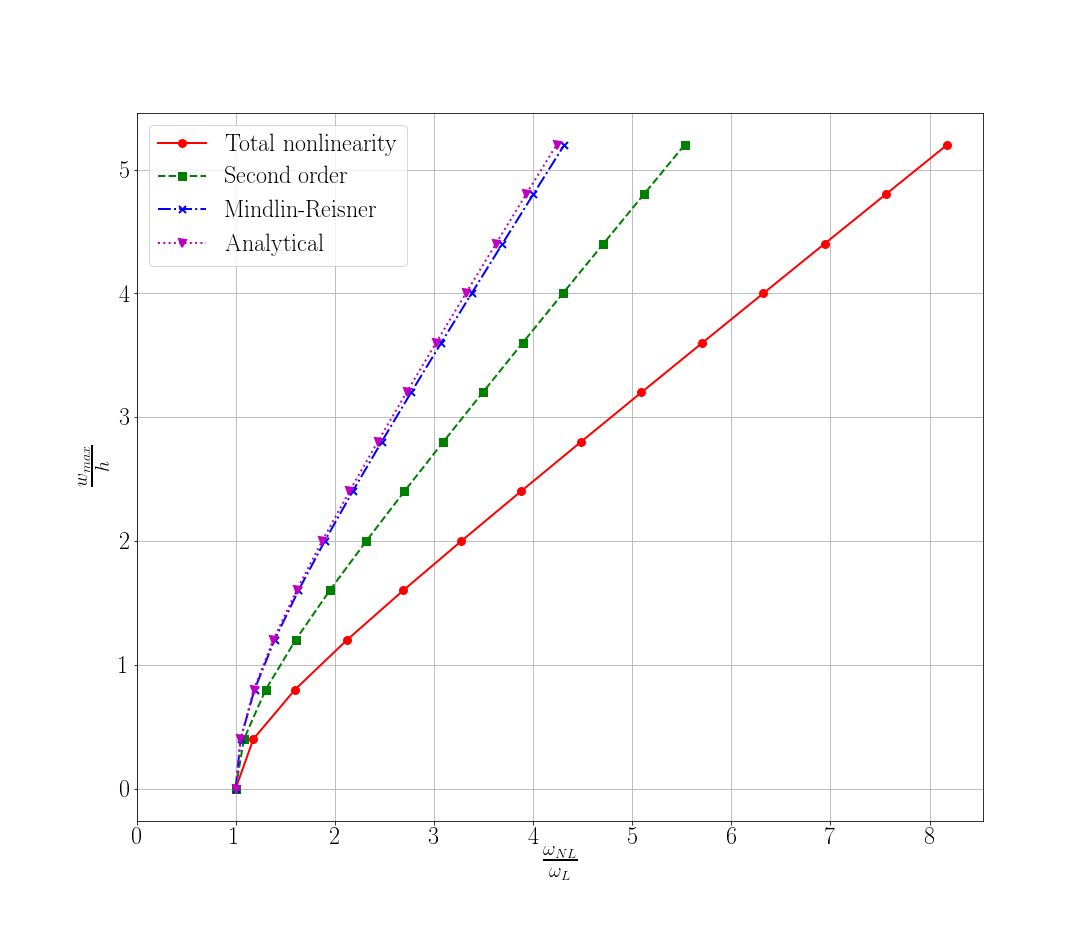
\includegraphics[scale=0.2]{pic/AFRC1.png}
		\caption{Амплітудно-частотні характеристики, отримані за допомогою узагальненого методу збурень для панелі, видовжені краї якої защемлені}
		\label{fig:AFR_C}
\end{figure}


\end{frame}

\begin{frame}{Розділ 4}

\begin{figure}
	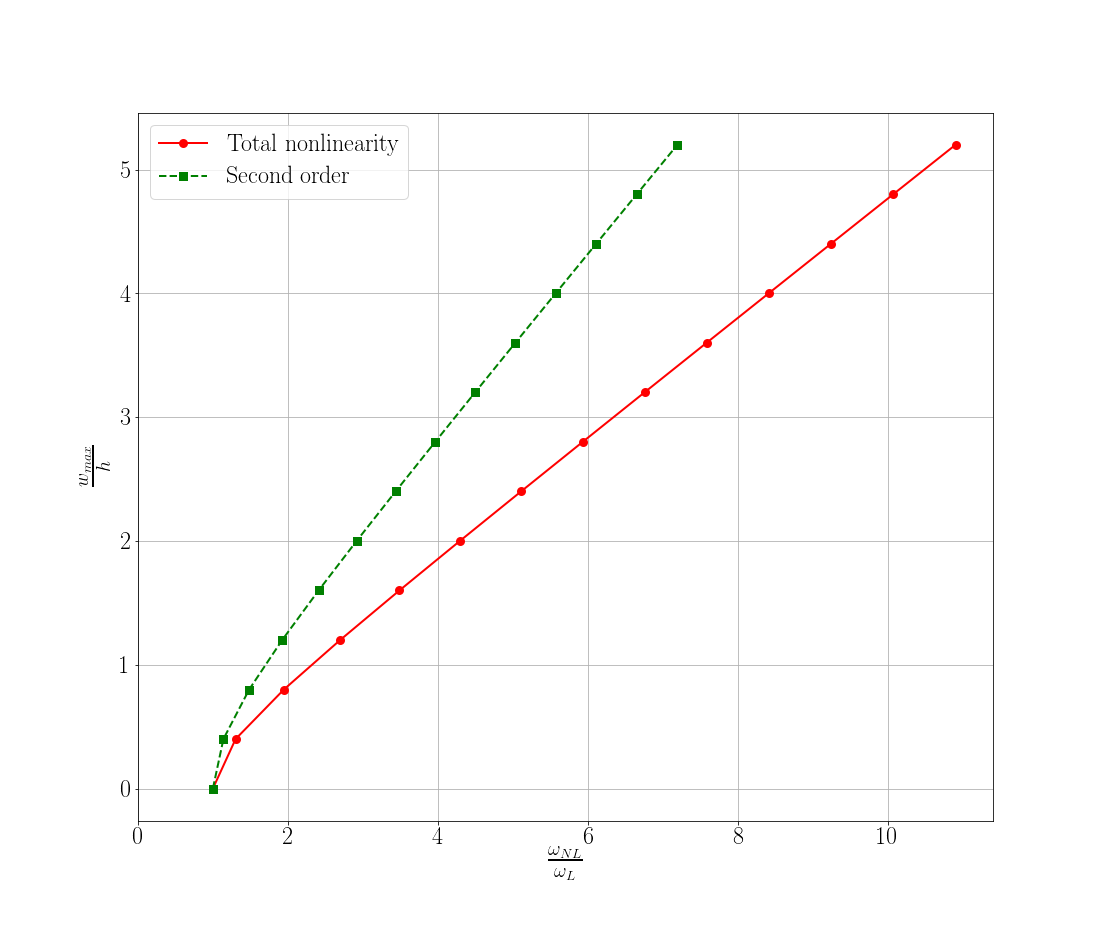
\includegraphics[scale=0.2]{pic/AFRC2.png}
		\caption{Амплітудно-частотні характеристики, отримані за допомогою вдосконаленого методу збурень для панелі, видовжені краї якої закріплені на нерухомих шарнірах}
		\label{fig:AFR_H}
\end{figure}


\end{frame}

\begin{frame}{Розділ 4}
\textbf{\textit{4.1.2 Тришарова пластина-смуга}}
\\
Умови контакту між шарами
\begin{gather}
u_i^{(k-1)}\left(\alpha_1, h_{k-1},t \right)=u_i^{(k)}\left(\alpha_1, h_{k},t \right),\\
S^{(k-1)3i}\left(\alpha_1, h_{k-1},t \right)=S^{(k)3i}\left(\alpha_1, h_{k},t \right),
\end{gather}
\[ i=1,3, \alpha_1 \in [0;L], k=2,\dots,N.\]
Граничні умови на лицевих площинах панелі
\begin{equation}
S^{(m)31}\left(\alpha_1, h_{m},t \right)=S^{(m)33}\left(\alpha_1, h_{m},t \right)=0,\alpha_1 \in [0;L], m=0,N.
\end{equation}
Розглянуто пластину з геометричним та механічними характеристиками
\begin{gather*}
L=1\text{м}, h=0.1\text{м};\\
\text{Гума:}\qquad
E_1=E_3=210\cdot 10^{9} Па, v_{13}=v_{31}=0.3, \rho=8000 кг/м^3;\\
\text{Сталь:}\qquad
E_1=E_3=0.1\cdot 10^{9} Па, v_{13}=v_{31}=0.48, \rho=1200 кг/м^3.
\end{gather*}


\end{frame}


\begin{frame}{Розділ 4}

\begin{figure}
	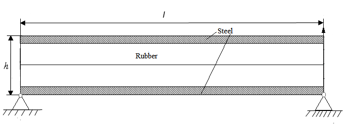
\includegraphics[scale=0.5]{pic/plate3layers.png}
		\caption{Тришарова пластина-смуга з нерухомими шарнірами на нижніх ребрах видовжених країв}
\end{figure}
\begin{table}[h!]
\centering
 \begin{tabular}{| c | c | c | c | c | c | c | c |} 
 \hline
 $\displaystyle \frac{h_{r}}{h}$ & 1 & 0.95 & 0.9 & 0.8 & 0.6 & 0.4 & 0 \\ 
  \hline
 $\omega_0$, Гц & 25.061 & 72.121 & 69.587 & 69.056 & 84.453 & 111.765 & 375.763 \\
   \hline
\end{tabular}
\caption{Вплив товщини шару гуми ($h_{r}$) на мінімальну власну частоту}
\label{table:2}
\end{table}

\begin{table}[h!]
\centering
 \begin{tabular}{| c | c | c | c | c | c | c | c |} 
 \hline
 $\displaystyle \frac{h_{r}}{h}$ & 1 & 0.95 & 0.9 & 0.8 & 0.6 & 0.4 & 0 \\ 
  \hline
 $R$, Гц & 16.1053 & 44.0470 & 73.2043 & 104.7005 & 92.1796 & 59.2721 & 5.7266 \\
   \hline
\end{tabular}
\caption{Вплив товщини шару гуми ($h_{r}$) на значення параметра нелінійності $R$}
\label{table:3}
\end{table}

\end{frame}

\begin{frame}{Розділ 4}

\begin{figure}
	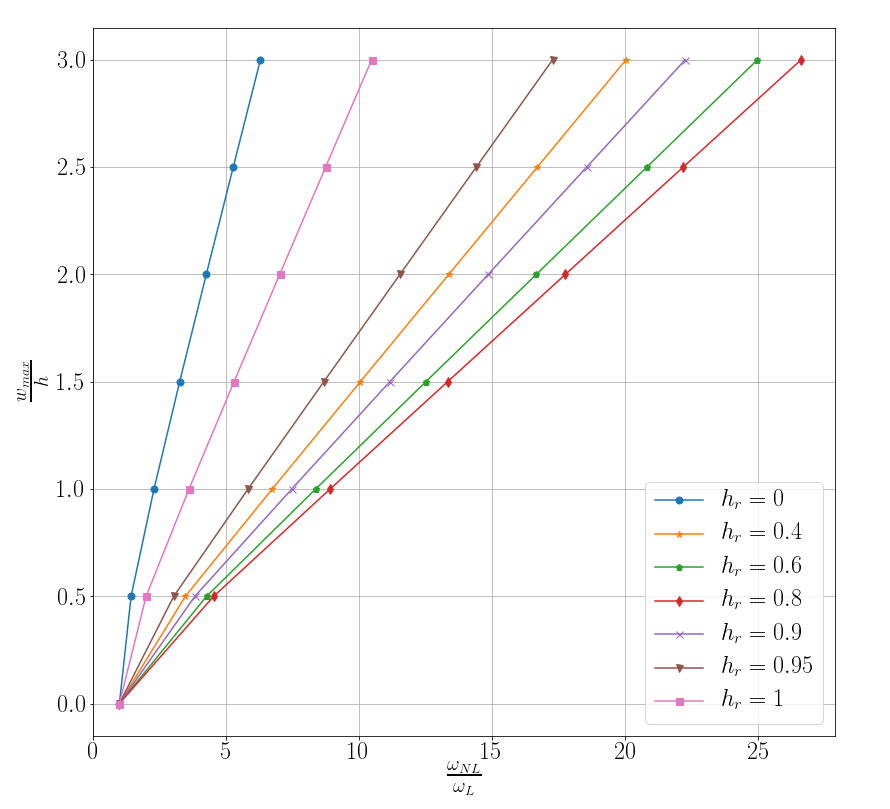
\includegraphics[scale=0.2]{pic/AFR_layered2.png}
		\caption{Амплітудно-частотні характеристики для тришарової панелі з нерухомими шарнірами на видовжених краях для різних значень $h_{r}$}
		\label{fig:AFR_layers}
\end{figure}


\end{frame}

\begin{frame}{Розділ 4}
\textbf{4.2. Видовжена циліндрична панель}
\begin{equation}
A\left( \alpha_1 \right)=1, \quad K\left( \alpha_1 \right)=\frac{1}{R}.
\end{equation}
\begin{figure}
	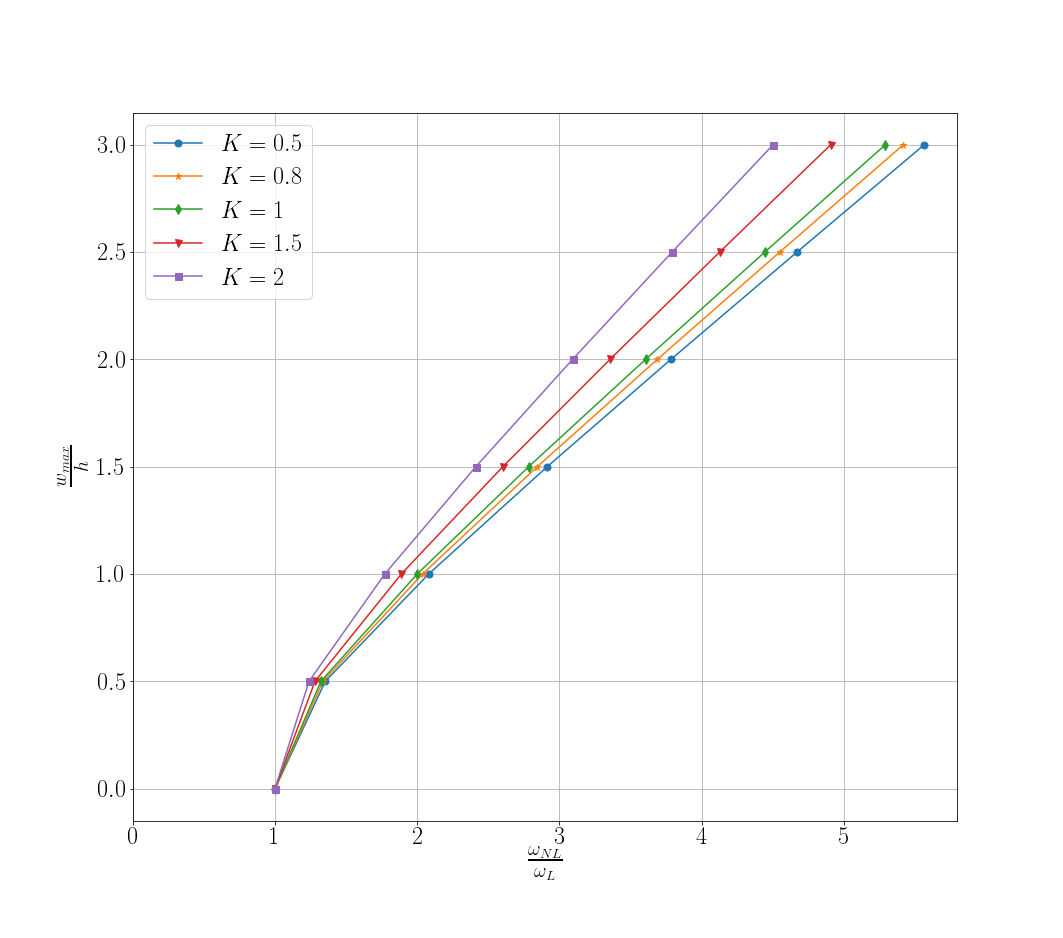
\includegraphics[scale=0.2]{pic/AFR_curvature.png}
		\caption{Амплітудно-частотні характеристики для панелі з вуглепластика з для різних значень кривини напрямної $K$}
		\label{fig:AFR_layers}
\end{figure}

\end{frame}

\begin{frame}{Розділ 4}

\begin{figure}[h]
\begin{minipage}[h]{0.49\linewidth}
\center{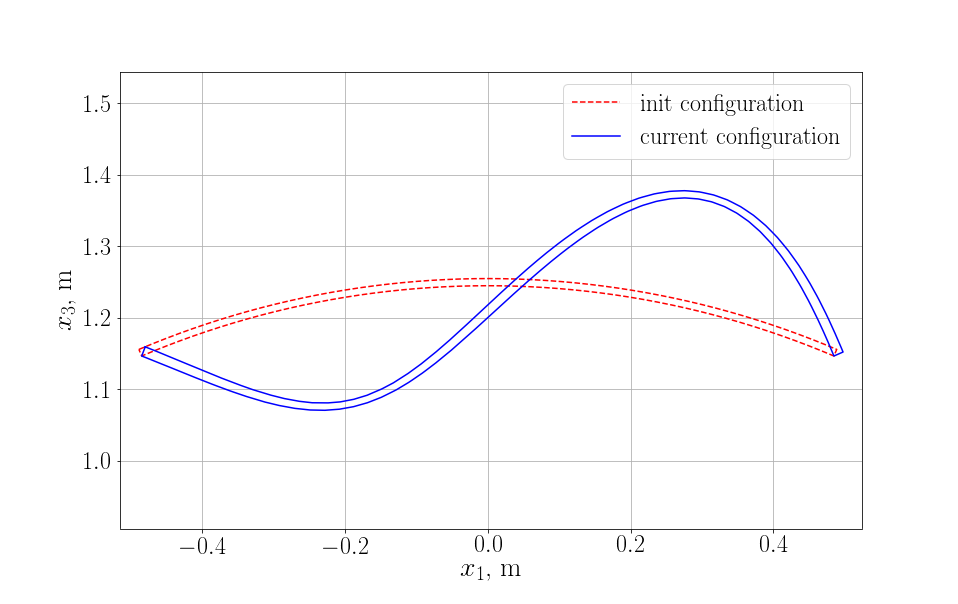
\includegraphics[width=\linewidth]{pic/def_K_08.png} \\ а)}
\end{minipage}
\hfill
\begin{minipage}[h]{0.49\linewidth}
\center{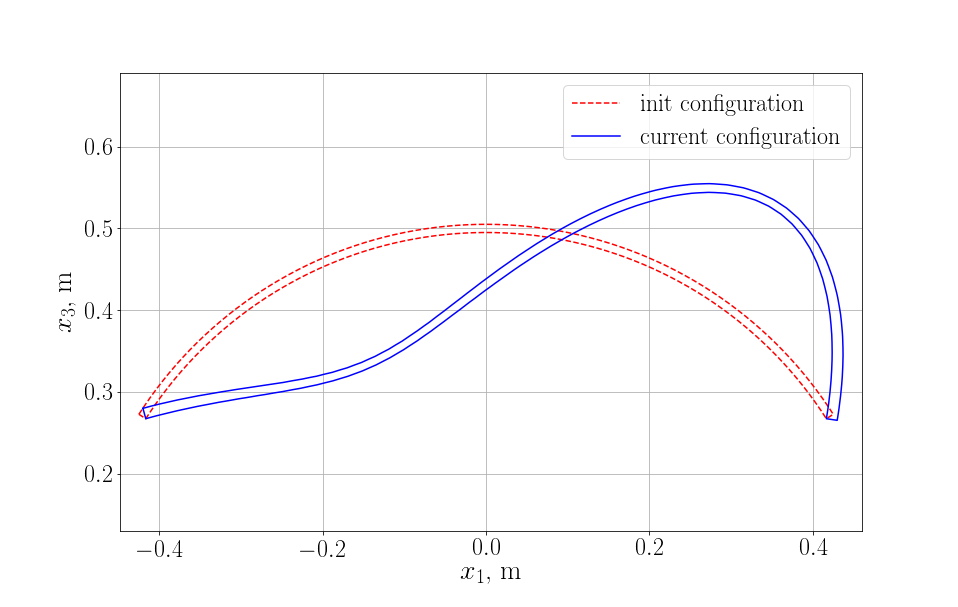
\includegraphics[width=\linewidth]{pic/def_K_2.png} \\ б)}
\end{minipage}
\caption{Перша мода циліндричної панелі з вуглепластику для різної кривизни: а)$K=0.8\text{м}^{-1}$; б)   $K=2\text{м}^{-1}$;}
\end{figure}

\end{frame}

\begin{frame}{Розділ 4}

\begin{figure}[h]
\begin{minipage}[h]{0.49\linewidth}
\center{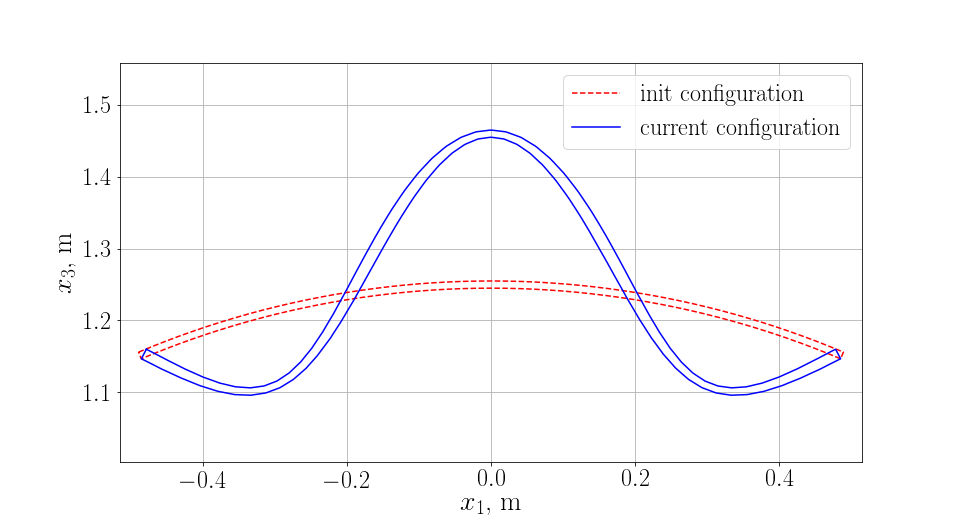
\includegraphics[width=\linewidth]{pic/def_K_08_2.png} \\ а)}
\end{minipage}
\hfill
\begin{minipage}[h]{0.49\linewidth}
\center{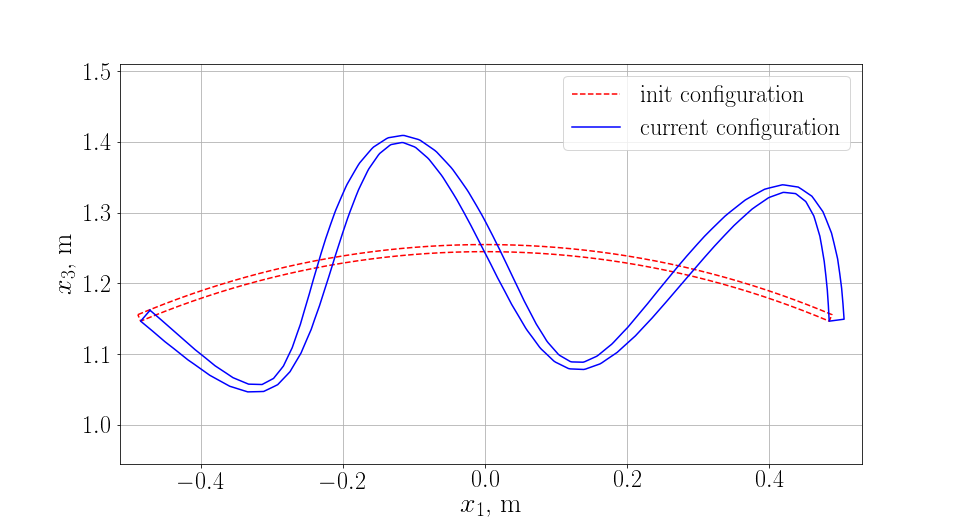
\includegraphics[width=\linewidth]{pic/def_K_08_3.png} \\ б)}
\end{minipage}
\caption{Вигляд циліндричної панелі $K=0.8\text{м}^{-1}$ з вуглепластику в різних модах: а) – перша мода; б) – друга;}
\end{figure}

\end{frame}

\begin{frame}{Розділ 4}

\begin{figure}
	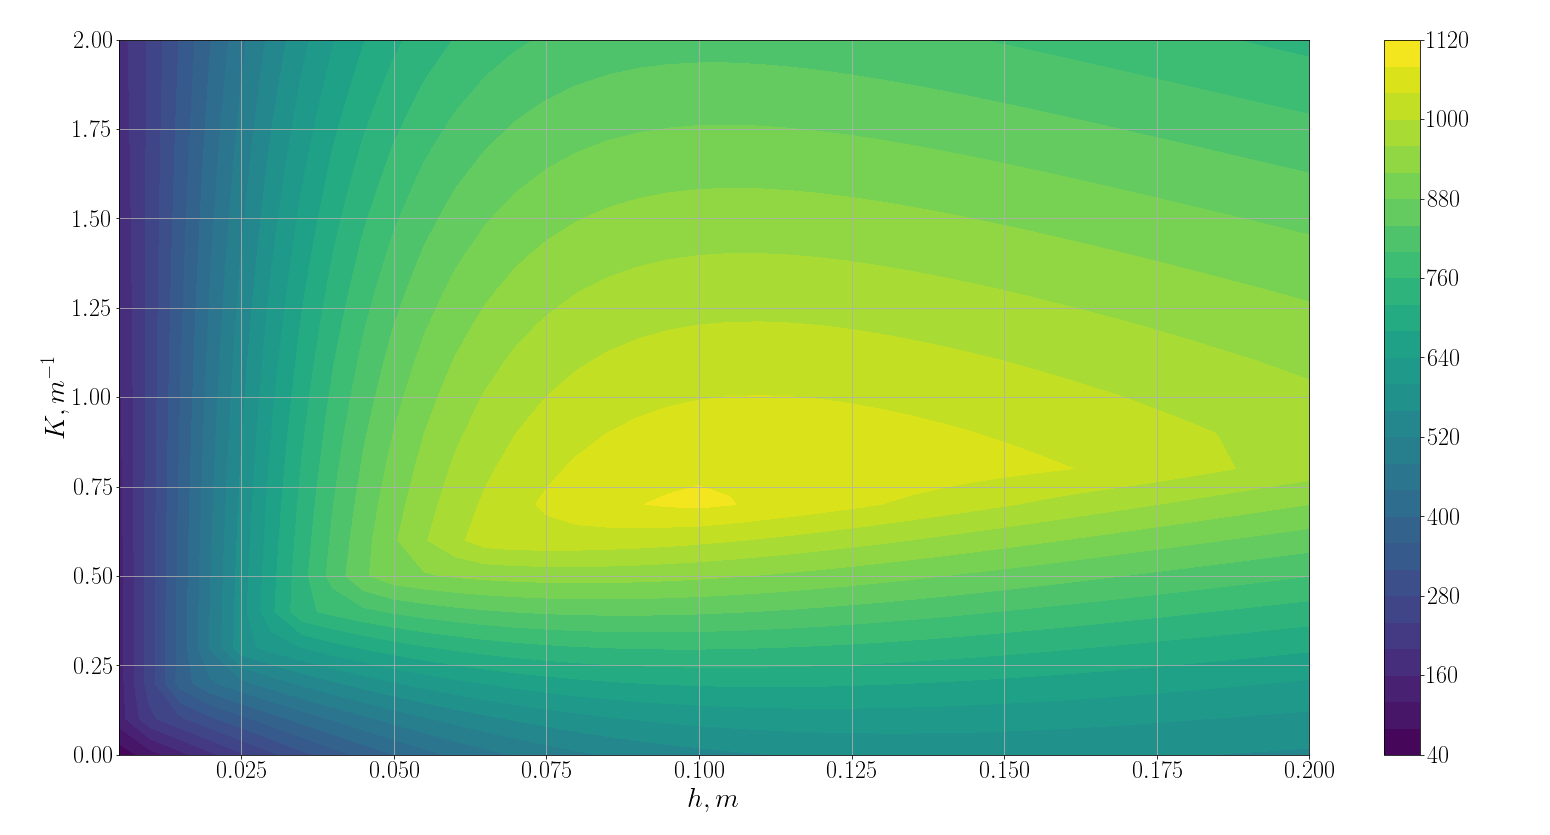
\includegraphics[scale=0.2]{pic/thickness_curvature_contour_plot2.png}
		\caption{Залежність найменшої власної частоти від радіуса кривини $K$ і товщини $h$ циліндричної панелі}
		\label{fig:omage_K_h}
\end{figure}

\end{frame}

\begin{frame}{Розділ 4}
\textbf{Висновки до розділу 4}\\
\vspace{1em}
\begin{itemize}
\item На основі розробленого алгоритму (методики) досліджено лінійні і геометрично нелінійні коливання одношарових та тришарових пластин-смуг.
\item Отримані числові результати дозволили встановити його ефективність шляхом його порівняння з розв'язками, отриманими іншими авторами.
\item Досліджено вплив податливості до трансверсьного зсуву на мінімальну власну частоту одношарової пластини-смуги.
\item Отримано аналітичну формулу для обчислення першої власної частоти за нелінійних коливань одношарової пластини смуги через значення лінійної власної частоти, нелінійної матриці жорсткості та лінійних власних векторів.
\item У випадку тришарової пластини смуги, що складається двох металевих лицевих та гумового середнього елементів, встановлено, що зі зростанням товщини гумового шару, мінімальна лінійна власна частота спадає. Встановлено, що максимальне значення нелінійної  першої власної частоти досягається при 80\% заповнені пластини смуги гумовим складником. 
\item Для циліндричної панелі встановлено, що зі зростанням кривизни вона стає менш жорсткою за нелінійних коливань. 
\end{itemize}

\end{frame}

\section{РОЗДІЛ 5}

\begin{frame}{РОЗДІЛ 5. ВІЛЬНІ КОЛИВАННЯ ГОФРОВАНИХ ПЛАСТИН СМУГ ТА ВИДОВЖЕНИХ ЦИЛІНДРИЧНИХ ПАНЕЛЕЙ.}
\textbf{5.1. Геометричні співвідношення і базові вектори для видовженої циліндричної панелі з гофруванням}
\\
\vspace{1em}
\begin{align}
x_1&=\left(R + g_{A}\cos\left(g_v\theta\right) \right)\cos\left(\theta\right), \\
x_2&=\alpha_2,\\
x_3&=\left(R + g_{A}\cos\left(g_v\theta\right) \right)\sin\left(\theta\right), 
\end{align}

\begin{tabbing}
де \= $L$ --- довжина напрямної циліндричного шару,\\
\> $R$ --- відстань від осі панелі до напрямної циліндричного шару,\\
\> $h$ --- товщина гофрованого шару,\\
\> $g_A$ --- амплітуда гофрування,\\
\> $g_v$ --- частота гофрування,\\
\end{tabbing}
\[
\theta=\theta\left(\alpha_1\right)=\frac{\pi}{2}+\frac{1}{R}\left(\frac{L}{2}-\alpha_1\right)\]


\end{frame}

\begin{frame}{Розділ 5}

\begin{figure}
	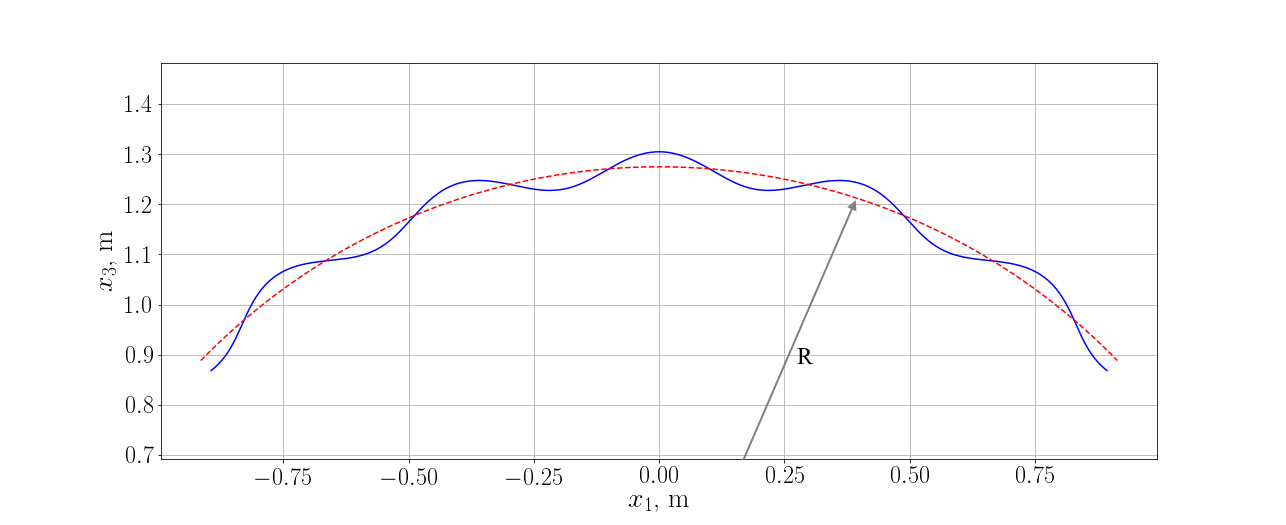
\includegraphics[width=0.8\linewidth]{pic/cor_geomR.png}\\
	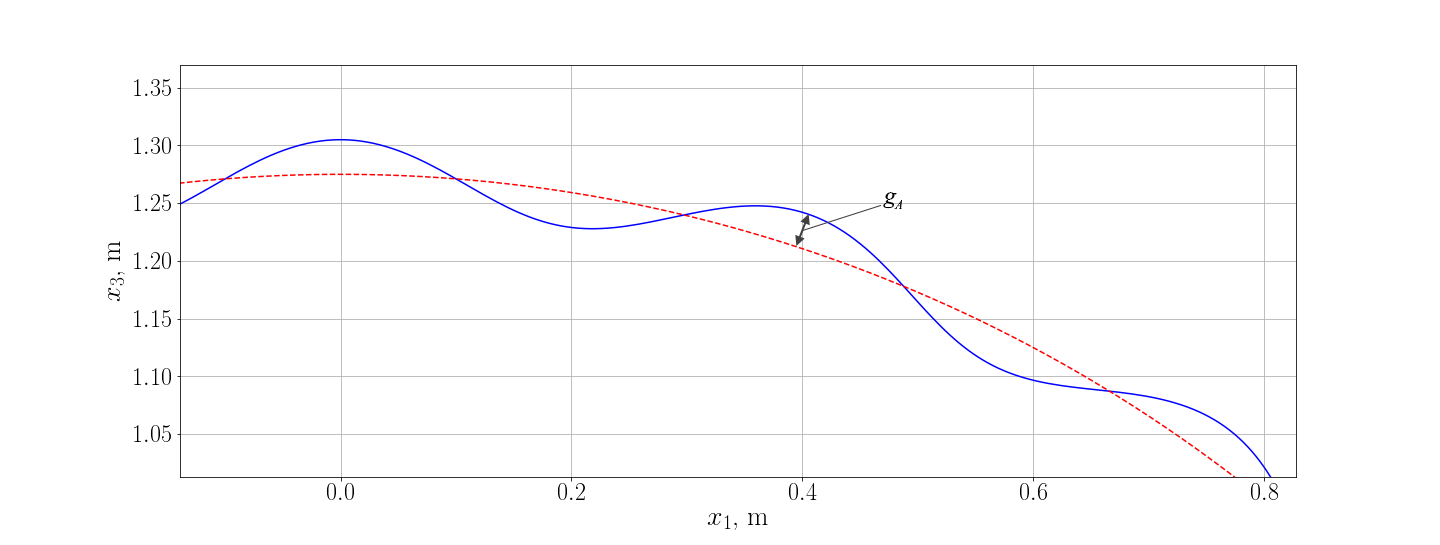
\includegraphics[width=0.8\linewidth]{pic/cor_geom_zoomedR.png}
		\caption{Напрямна серединної поверхні шару в декартовій системі координат за $g_v=20$.}
		\label{fig:omage_K_h}
\end{figure}



\end{frame}

\begin{frame}{Розділ 5}
\begin{figure}
	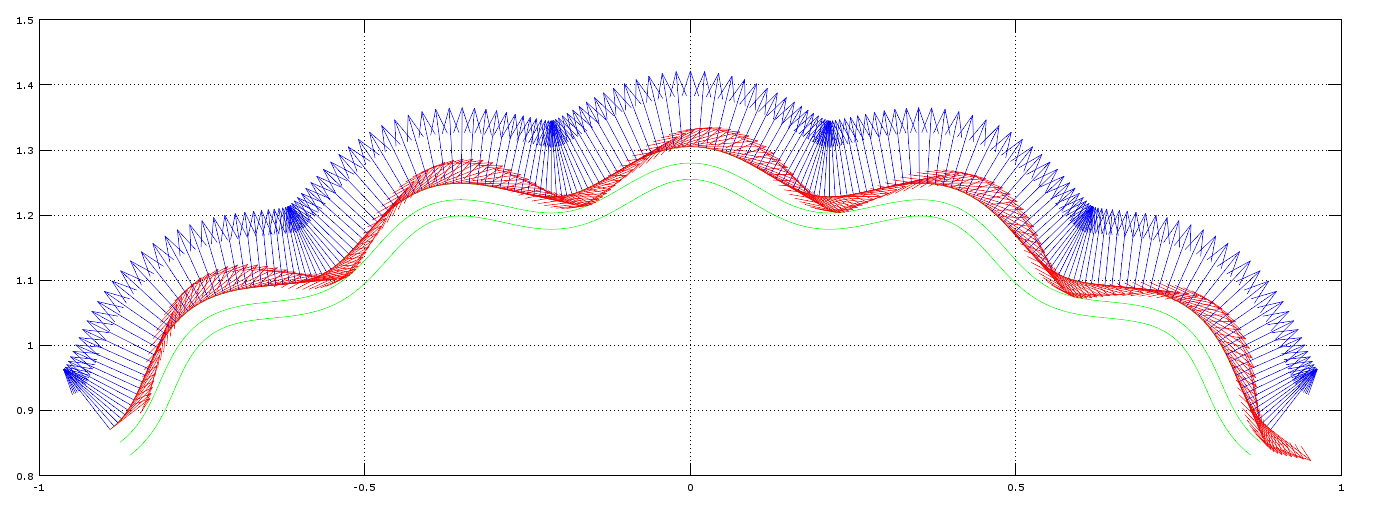
\includegraphics[scale=0.2]{pic/cor_R1R32.png}
		\caption{Вектори коваріантної бази $\vec{R}_1$ (червоний колір) і $\vec{R}_3$ (синій колір) на верхній лицевій поверхні $L=2\text{м}, h=0.05\text{м},R=1.25\text{м},g_A=0.03\text{м}, g_v=20$.}
\end{figure}

Радіус вектор до будь-якої точки панелі
\begin{equation}
\vec{R}=\vec{r}+\alpha_3\vec{n},
\end{equation}
\begin{tabbing}
де \= $\vec{r} = x_1\vec{e}_1+x_2\vec{e}_2+x_3\vec{e}_3$ --- радіус вектор до серединної поверхні,\\
\> $\vec{n}$ --- нормаль до серединної поверхні.
\end{tabbing}

Вектори коваріантної бази локальної системи координат
\begin{align}
\vec{R}_1&=\frac{\partial \vec{r}}{\partial \alpha_1}+\alpha_3\frac{\partial \vec{n}}{\partial \alpha_1},\\
\vec{R}_2 &= \vec{e}_2,\\
\vec{R}_3 &= \vec{n}.
\end{align}

\end{frame}

\begin{frame}{Розділ 5}
Коефіцієнт першої квадратичної форми і головна кривизна
\begin{gather}
A\left(\alpha_1\right) = \sqrt{w^2+z^2},\\
K\left(\alpha_1\right) = \frac{\left(wy+2z^2/R\right)}{A\left(\alpha_1\right)^{\frac{3}{2}}},
\end{gather}
де
\begin{gather*}
w=1+\frac{g_A}{R}\cos\left(g_v\theta\right),\\
z=\frac{g_A g_v}{R}\sin\left(g_v\theta\right),\\
y=-\frac{w}{R}+\frac{g_A g_v^2}{R^2}\cos\left(g_v\theta\right).
\end{gather*}

\end{frame}

\begin{frame}{Розділ 5}
\textbf{5.2. Геометрично нелінійні коливання.}
\\
\vspace{1em}
Геометричні та механічні  характеристики
\begin{gather*}
L=2\text{м}, h=0.05\text{м},R=1.25\text{м},g_A=0.03\text{м}, g_v=20,\\
E_1=E_3=2.1\cdot 10^{11} Па, v_{13}=v_{31}=0.3, G_{13}=8.1\cdot 10^{10} Па, \rho=8000 кг/м^3.
\end{gather*}
\begin{table}[h!]
\centering
\resizebox{\textwidth}{!}{
 \begin{tabular}{| c | c | c | c | c | c | c | c | c | c | c | c | c | c | c |} 
 \hline
 $g_v$ & 2 & 4 & 6 & 8 & 15 & 20 & 50 & 80 & 100 & 200 & 300 & 500 \\ 
  \hline
 $\omega$, Гц & 105 & 98 & 92 & 110 & 132 & 217 & 2588 & 8007 & 11138 & 20220 & 18239 & 12042\\
   \hline
\end{tabular}}
\caption{Залежність найменшої власної частоти ($\omega$) від частоти гофрування ($g_v$) панелі}
\label{table:51}
\end{table}

\begin{figure}[h]
\begin{minipage}[h]{0.49\linewidth}
\center{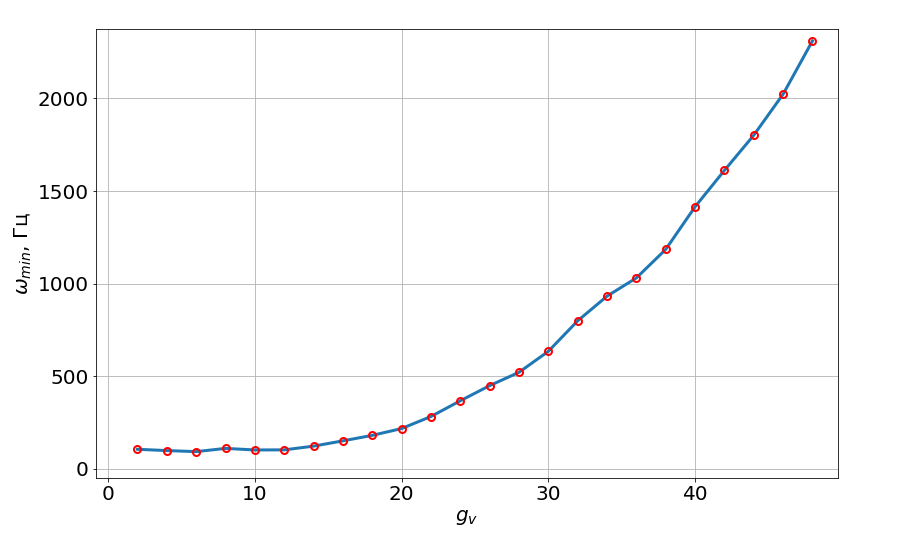
\includegraphics[width=\linewidth]{pic/gv_freq2.png} \\ а)}
\end{minipage}
\hfill
\begin{minipage}[h]{0.49\linewidth}
\center{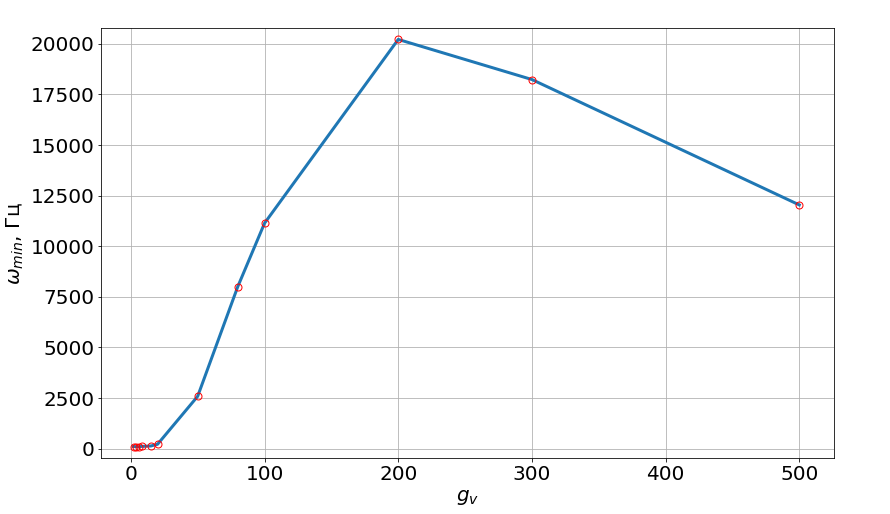
\includegraphics[width=\linewidth]{pic/gv_freq_ex.png} \\ б)}
\end{minipage}
\caption{Залежність найменшої власної частоти ($\omega$) від частоти гофрування ($g_v$) панелі}
\end{figure}
\end{frame}


\begin{frame}{Розділ 5}
\begin{figure}[h]
\begin{minipage}[h]{0.49\linewidth}
\center{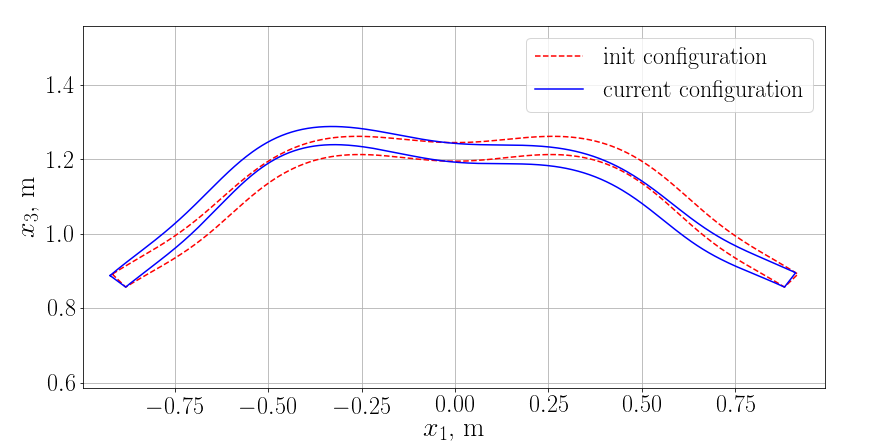
\includegraphics[width=\linewidth]{pic/corrugated_deforms_10.png} \\ а)}
\end{minipage}
\hfill
\begin{minipage}[h]{0.49\linewidth}
\center{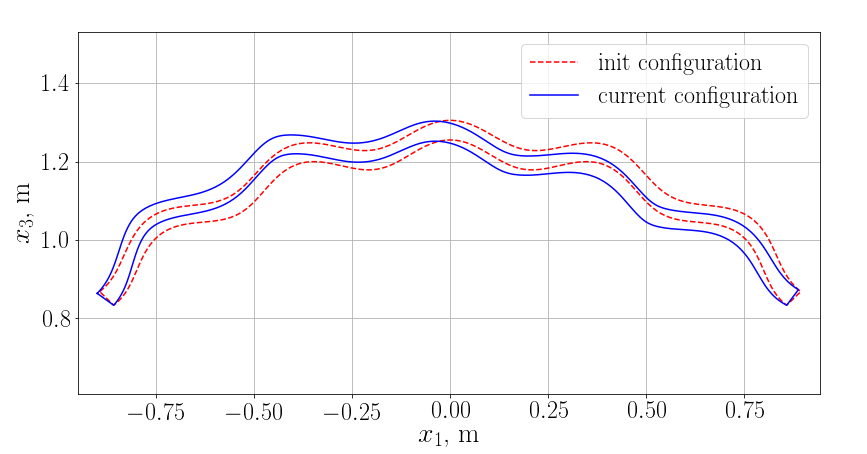
\includegraphics[width=\linewidth]{pic/corrugated_deforms_20.png} \\ б)}
\end{minipage}
\caption{Перша мода гофрованої циліндричної панелі з різними частотами гофрування: а) $g_v=10$; б)$g_v=20$.}
\end{figure}

\begin{figure}[h]
\begin{minipage}[h]{0.49\linewidth}
\center{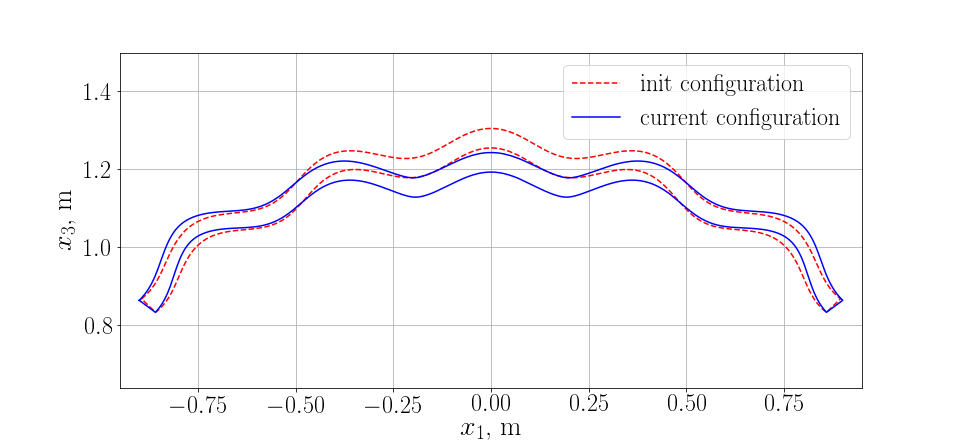
\includegraphics[width=\linewidth]{pic/corrugated_deforms_20_2.png} \\ а)}
\end{minipage}
\hfill
\begin{minipage}[h]{0.49\linewidth}
\center{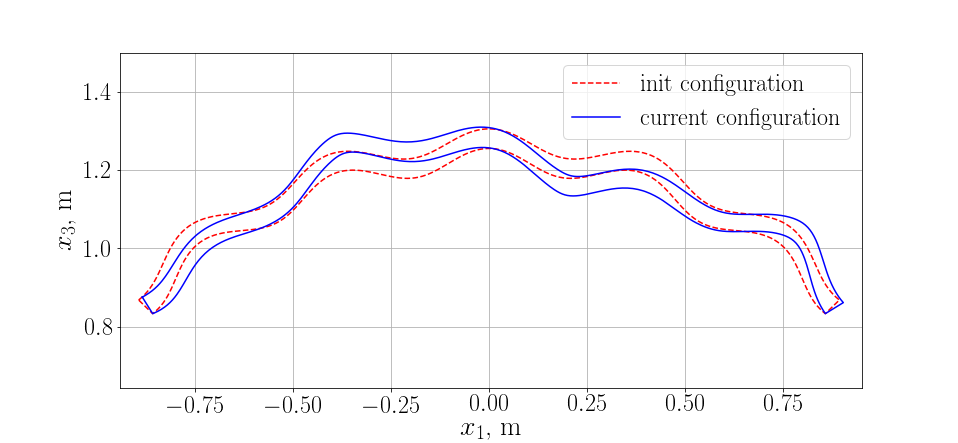
\includegraphics[width=\linewidth]{pic/corrugated_deforms_20_3.png} \\ б)}
\end{minipage}
\caption{Вигляд гофрованої циліндричної панелі в різних модах: а) перша; б) друга.}
\end{figure}
\end{frame}

\begin{frame}{Розділ 5}

\begin{figure}
	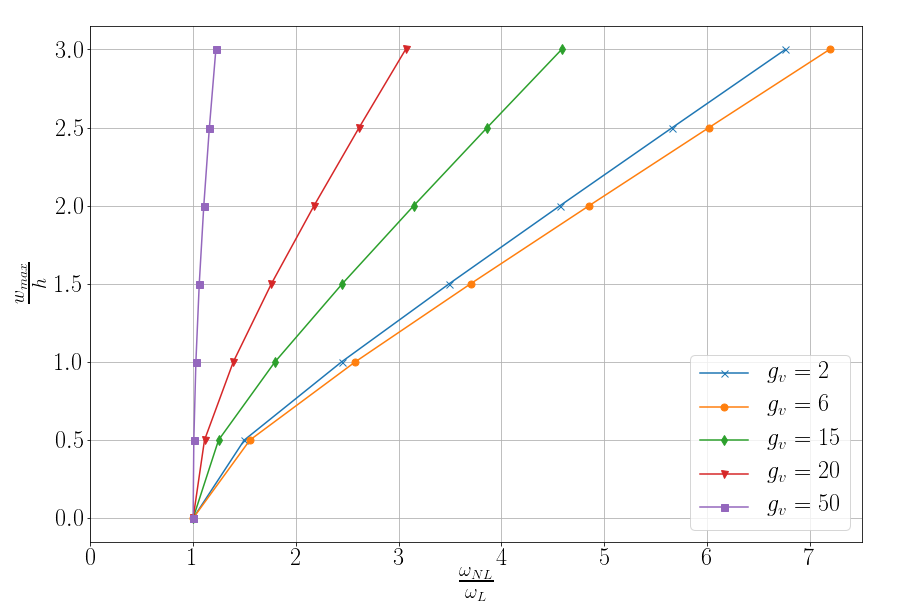
\includegraphics[scale=0.3]{pic/corrugated_nonlinear.png}
		\caption{Амплітудно-частотні характеристики гофрованої панелі для різних значень частоти гофрувань $g_v$.}
\end{figure}

\end{frame}

\begin{frame}{Розділ 5}
\begin{table}[h!]
\centering
\resizebox{\textwidth}{!}{
 \begin{tabular}{| c | c | c | c | c | c | c | c | c |} 
 \hline
 $g_A$, м & 0 & 0.015 & 0.03 & 0.06 & 0.1 & 0.2 & 0.25 & 0.3 \\ 
  \hline
 $\omega$, Гц & 101 & 143 & 217 & 377 & 622 & 675 & 552 & 461\\
   \hline
\end{tabular}}
\caption{Залежність найменшої власної частоти ($\omega$) від амплітуди гофрування ($g_A$) панелі.}
\label{table:51}
\end{table}

\begin{figure}
	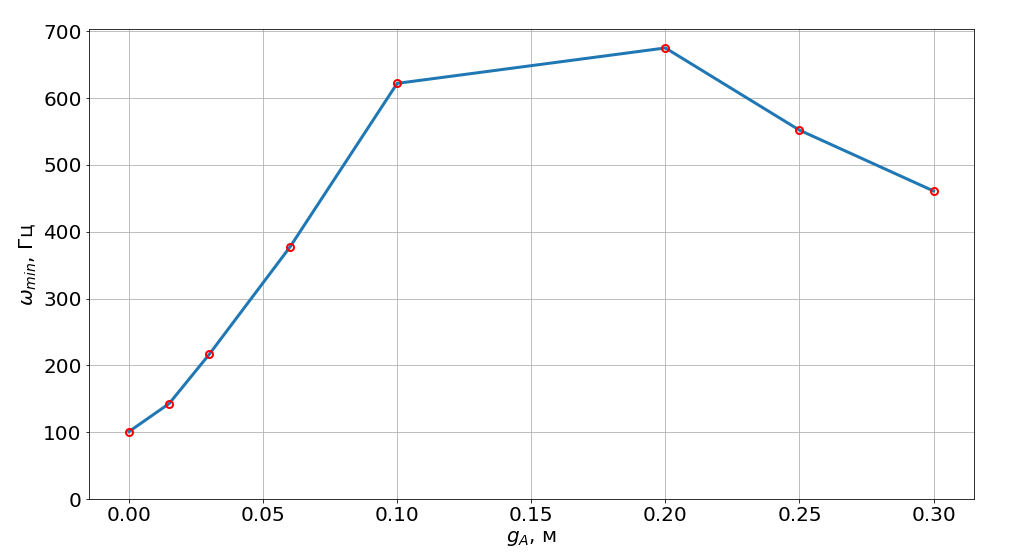
\includegraphics[scale=0.25]{pic/corrugated_ampl_linear.png}
		\caption{Залежність найменшої власної частоти ($\omega$) від амплітуди гофрування ($g_A$) панелі.}
\end{figure}
\end{frame}

\begin{frame}{Розділ 5}

\begin{figure}[h]
\begin{minipage}[h]{0.49\linewidth}
\center{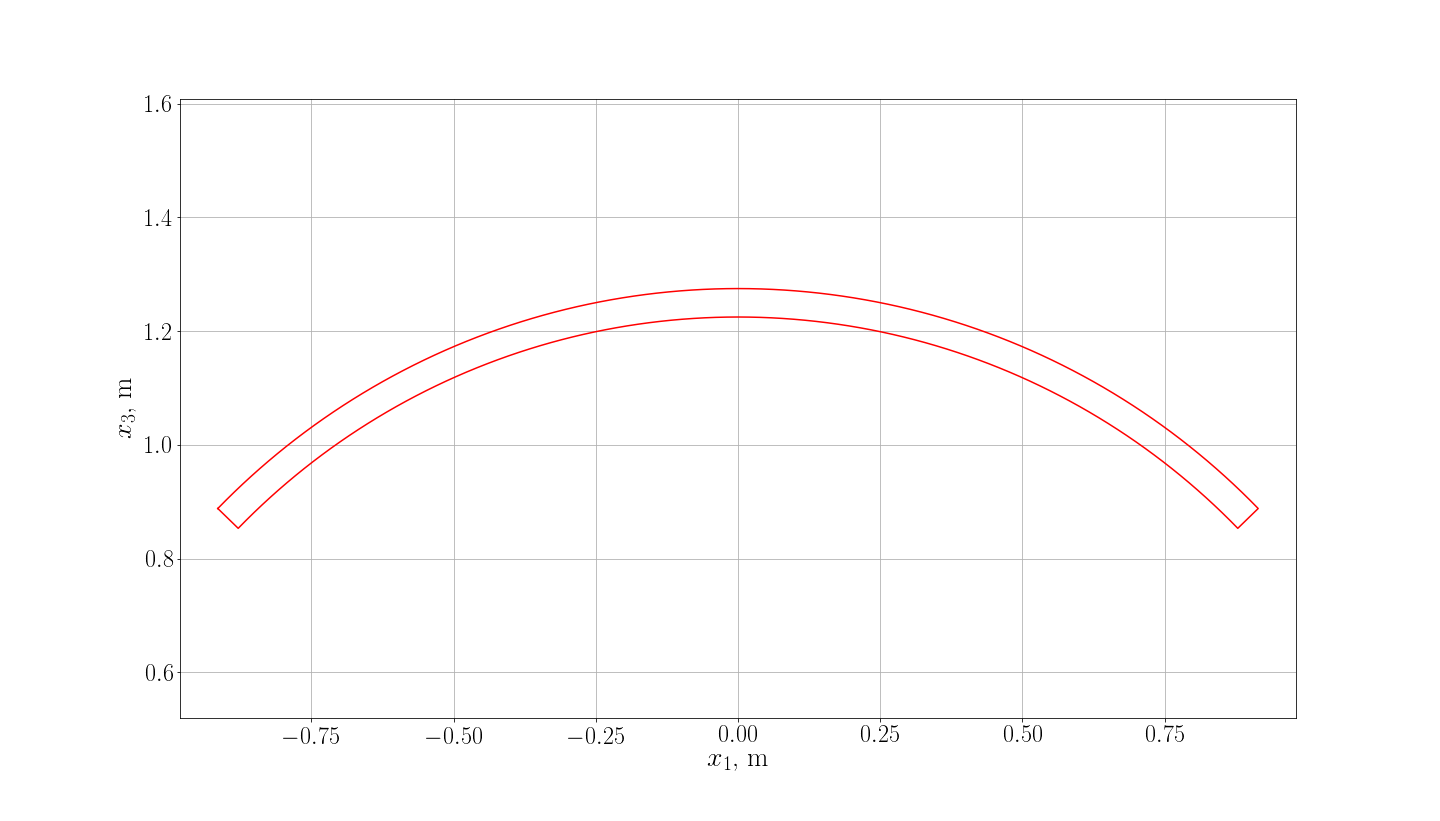
\includegraphics[width=\linewidth]{pic/cor_geom_ga0.png} \\ а)}
\end{minipage}
\hfill
\begin{minipage}[h]{0.49\linewidth}
\center{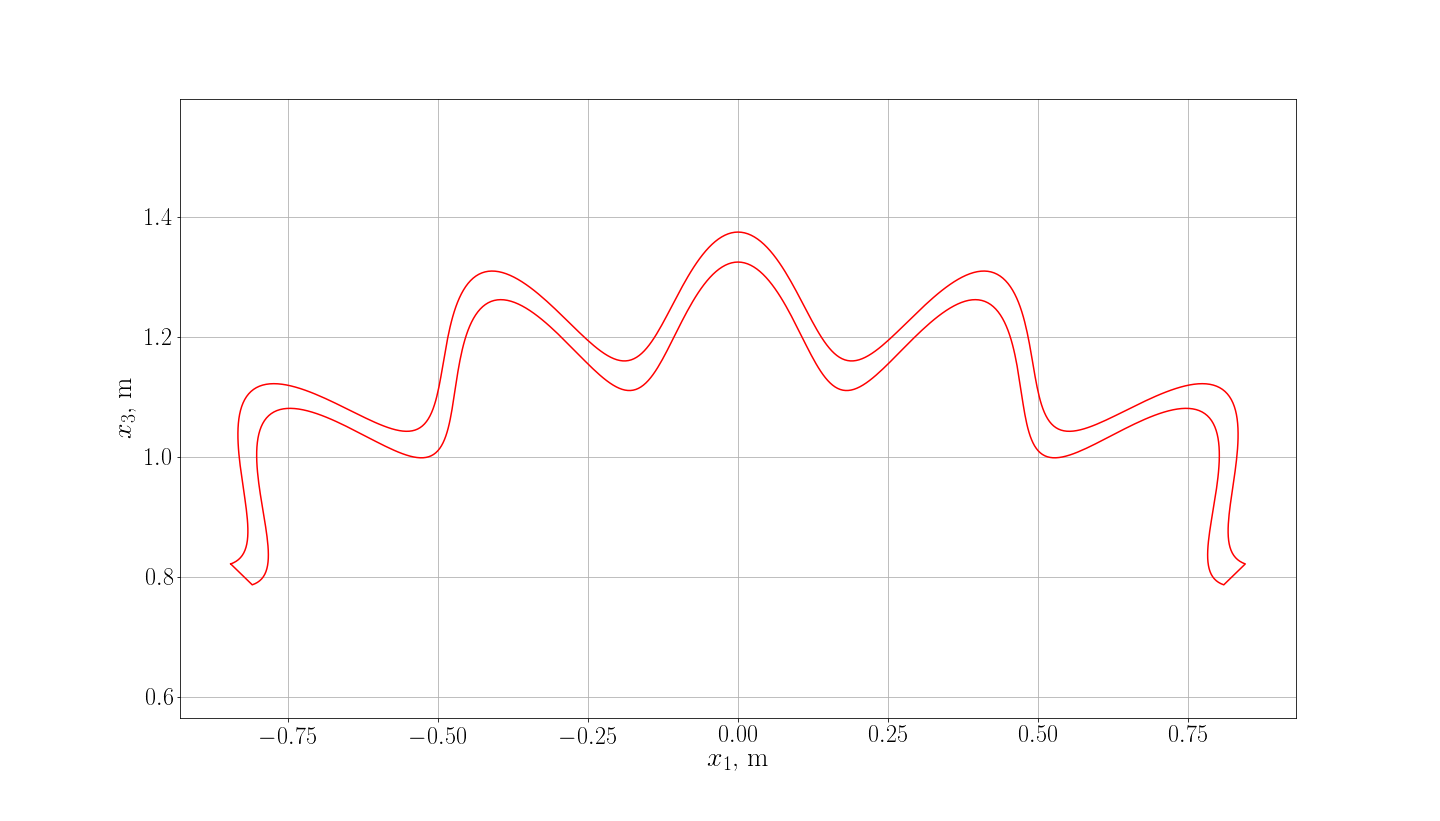
\includegraphics[width=\linewidth]{pic/cor_geom_ga01.png} \\ б)}
\end{minipage}
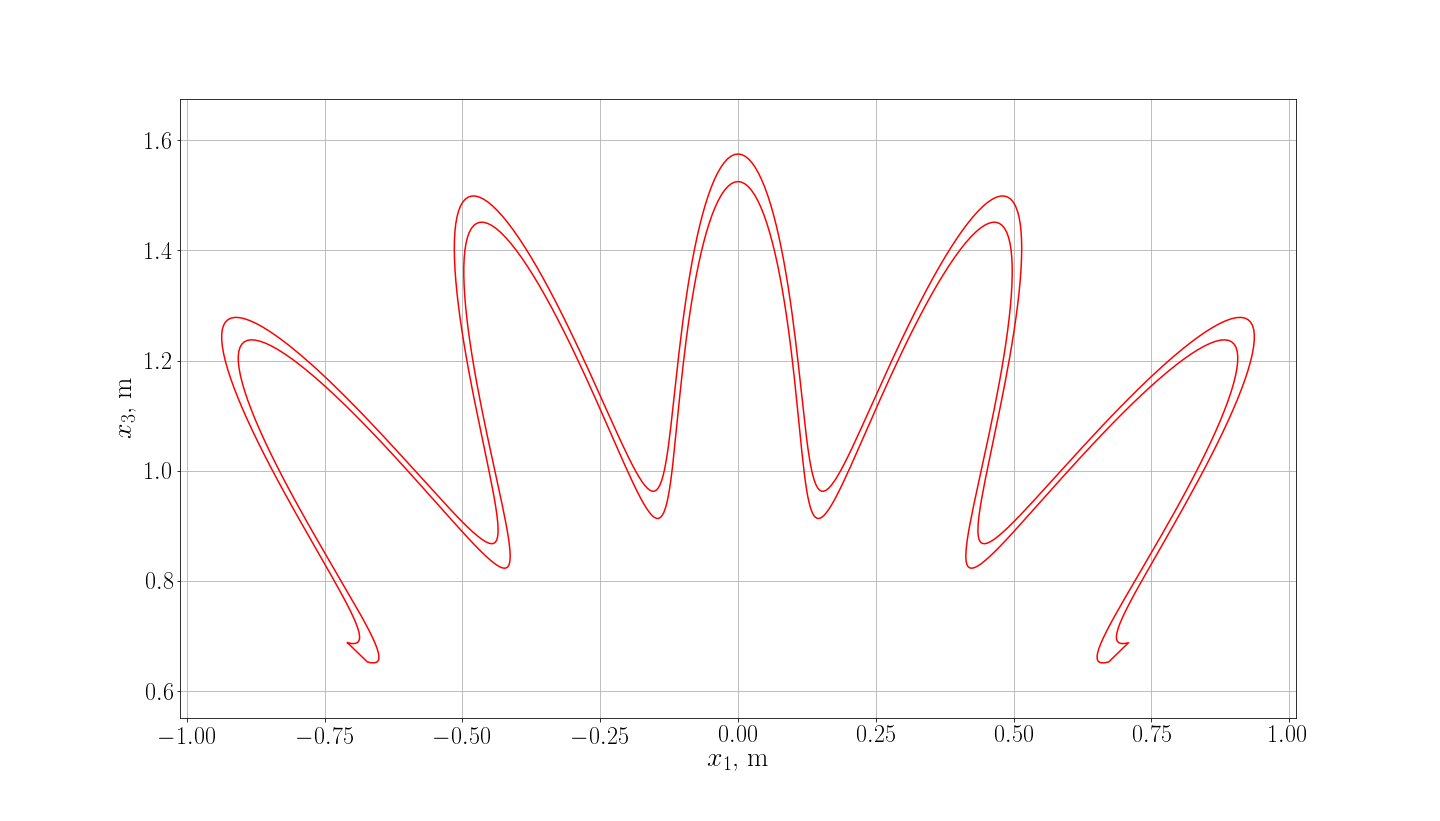
\includegraphics[width=0.49\linewidth]{pic/cor_geom_ga03.png} \\ в)
\caption{Вигляд гофрованої циліндричної панелі при \\а) $g_A = 0м$; б) $g_A = 0.1м$; в) $g_A = 0.3м$.}
\end{figure}

\end{frame}

\begin{frame}{Розділ 5}

\begin{figure}
	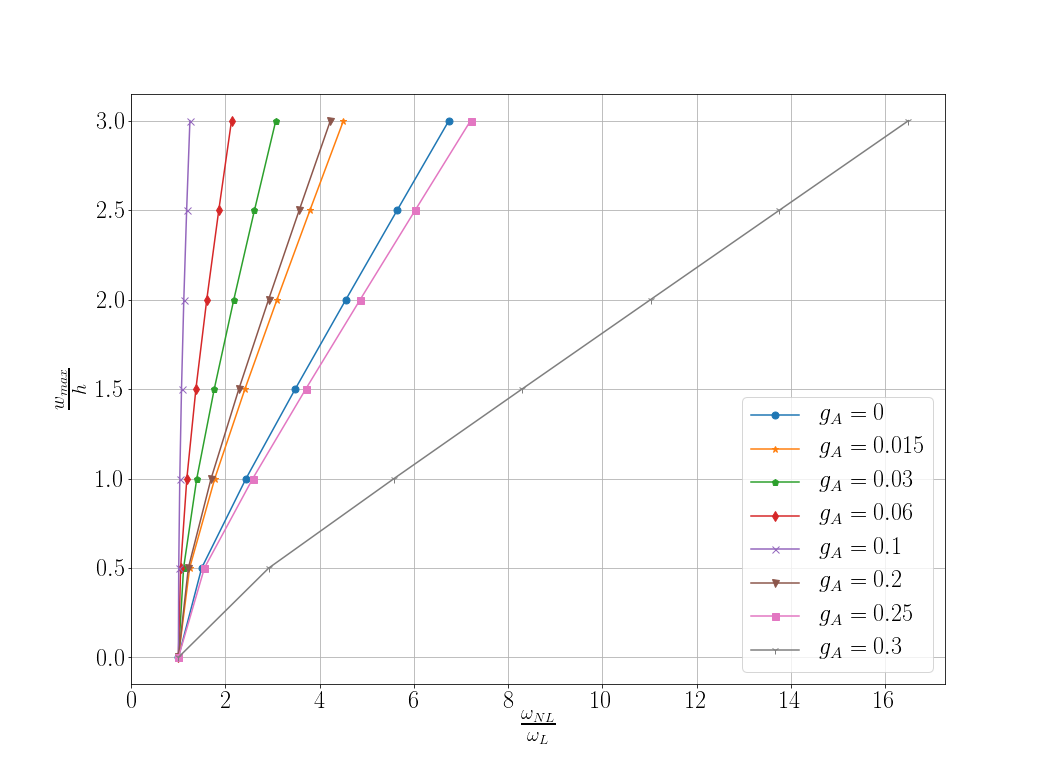
\includegraphics[scale=0.25]{pic/corrugated_ampl_nonlinear_s.png}
		\caption{Амплітудно-частотні характеристики гофрованої панелі для різних значень частоти гофрувань $g_А$.}
\end{figure}

\end{frame}

\begin{frame}{Розділ 5}
\textbf{Висновки до розділу 5}\\
\vspace{1em}
\begin{itemize}
\item Отримані співвідношення просторової геометрично нелінійної динамічної теорії пружності для гофрованого в колову напрямку циліндричного шару.
\item Досліджено вплив частоти гофрування на мінімальну власну частоту гофрованої в колову напрямку циліндричної оболонки.
\item Знайдено форми власних коливань гофрованої в колову напрямку циліндричної оболонки для різних значень частот.
\item Проаналізовані
\end{itemize}

\end{frame}

\end{document}